\chapter{Самокаталитические ННК GaP: кристаллическая структура и влияние
условий роста на морфологию массива}\label{ch:ch5}

GaP со структурой ZB~--- непрямозонный полупроводник с шириной запрещённой зоны
2,24~\si{\electronvolt}. Однако, введение в GaP относительно небольшого
количества азота (\(\approx 3,1\)\,\%) изменяет характер основного оптического
перехода от непрямозонного
(\(\Gamma\textsubscript{V}\)\,--\,\(X\textsubscript{C}\)) к прямозонному
переходу (\(\Gamma\textsubscript{V}\)\,--\,\(\Gamma\textsubscript{C}\))
\cite{shan2000, rudko2003}. Это преобразование объясняется в рамках модели
антипересечения зон и основано на взаимодействии между локализованными азотными
состояниями и состояниями \(\Gamma\textsubscript{C}\) минимума зоны
проводимости. GaPAs с концентрацией As более 51\,\% тоже является прямозонным
материалом \cite{polak2019}. Введение As и N в GaP в различных концентрациях
позволяет изменять ширину запрещённой зоны в диапазоне
1,5--2,24~\si{\electronvolt}, что покрывает спектральный диапазон от
жёлто-зелёного до ближнего инфракрасного \cite{bellaiche1997}.

Получить прямозонный материал можно не только добавлением примесей: GaP со
структурой WZ~--- также прямозонный полупроводник с шириной запрещённой зоны
2,18--2,25~\si{\electronvolt} \cite{Assali2016}. Данная структура нестабильна
при нормальных условиях в объёмных материалах, однако была стабилизирована в
ННК, выращенных с применением Au катализатора \cite{Husanu2014}.

Для фундаментальной науки GaP ННК интересны из-за возможности формирования
осевых и радиальных гетероструктур с резким изменением электронных свойств
материала, а для практического применения~--- перспективой создания
красно-жёлтых светоизлучающих диодов для гибкой электроники и миниатюрных
лазерных излучателей.

В данной главе излагается результат исследования формирования
самокаталитических ННК GaP на подложках Si(111) методом МПЭ. Показано влияние
состояния поверхности и ростовых параметров на рост паразитных островков,
поверхностную плотность и ориентацию ННК.

\section{Постановка эксперимента}\label{sec:ch5/sec1}

ННК GaP синтезированы по механизму ПЖК на установке МПЭ Veeco GEN III на
подложках Si(111). Потоки Ga представлены относительно потока, который
соответствует планарной скорости роста GaP/Si(001)
180~\si{\nano\meter\per\hour} в избытке P. Отношение ЭДП P\textsubscript{2}/Ga,
соответствующее стехиометрическому отношению адатомов на поверхности подложки,
равно 6, что определено по накоплению капель Ga с меньшим отношением ЭДП
P\textsubscript{2}/Ga при росте планарного GaP на Si(001) (при температуре
580~\si{\degreeCelsius} и потоке Ga соответствующем скорости роста
180~\si{\nano\meter\per\hour}).

Использовались вицинальные (разориентация 4{\textdegree} в направлении [110]) и
сингулярные (\(\pm 0,1\){\textdegree}) подложки Si(111). Очистка подложек по
модифицированному методу Шираки \cite{Okumura1997, Ishizaka2019} оканчивалась
окислением в кипящем растворе
H\textsubscript{2}O\textsubscript{2}:NH\textsubscript{4}OH:H\textsubscript{2}O
в соотношении 1:1:3 или в азеотропной смеси
HNO\textsubscript{3}:H\textsubscript{2}O (68\,\% HNO\textsubscript{3},
температура кипения \(\approx 120\)~\si{\degreeCelsius}) \cite{Imamura2010}.

После дегазации в загрузочной и буферной камерах установки МПЭ подложки Si(111)
отжигались в течение 30~\si{\minute} при температуре на 30~\si{\degreeCelsius}
ниже, чем температура быстрого термического разложения SiO\textsubscript{x}.
Отжиг проводился с целью утонения оксида, что ведёт к уменьшению смачиваемости
поверхности \cite{Matteini2015}, что, в свою очередь, способствует образованию
таких капель Ga катализатора, которые приводят к росту плотного массива
вертикальных самокаталитических ННК GaP \cite{Dubrovskii2012a}.

Крекинговые источники могут проявлять инерционность в стабилизации потока,
особенно после длительного стояния с закрытым клапаном, а регулировка положения
игольчатого клапана может занимать несколько секунд. Чтобы сократить переходные
процессы во время стабилизации потока игольчатый клапан источника P
настраивался на требуемое положение за 20~\si{\second} до открытия заслонки
источника. В этот период времени попадающий на подложку ЭДП P\textsubscript{2}
не превышал \(4 \cdot 10^{-7}\)~\si{\torr}.

Морфология синтезированных массивов ННК изучена методом РЭМ (Zeiss SUPRA 25).
Кристаллическая структура исследована методом ПРЭМ на микроскопе JEOL
JEM-ARM200F Cold FEG ПЭМ/ПРЭМ с ускоряющим напряжением 200~\si{\kilo\volt}.
Микроскоп оснащён додекапольными корректорами сферических аберраций
(Cs-корректоры) (разрешение 0,19~\si{\nano\meter} в режиме ПЭМ и
0,078~\si{\nano\meter} в режиме ПРЭМ). Для исследований ПЭМ ННК были
механически отделены от подложки и перенесены на сетку с углеродным покрытием.

\section{Влияние состояния поверхностного SiO\textsubscript{x} и
предварительного нанесения Ga}\label{sec:ch5/sec2}

На рисунке \cref{fig:Image_38} изображены ННК из различных областей образца,
выращенного с градиентом температуры отжига поверхностного
SiO\textsubscript{x}, сформированного в растворе
HNO\textsubscript{3}:H\textsubscript{2}O. В случае низкой температуры отжига
(см.~рис.~\cref{fig:Image_38_1}) образуется большое количество наклонных ННК, а
в случае высокой (см.~рис.~\cref{fig:Image_38_3})~--- оксид десорбируется (что
подтверждается образованием реконструкции поверхности
Si\((111)7\)\(\times\)\(7\), формирование ННК подавляется, образуются только
срастающиеся островки.

\begin{figure}[ht] \centerfloat{ \subcaptionbox{\label{fig:Image_38_1}}{%
		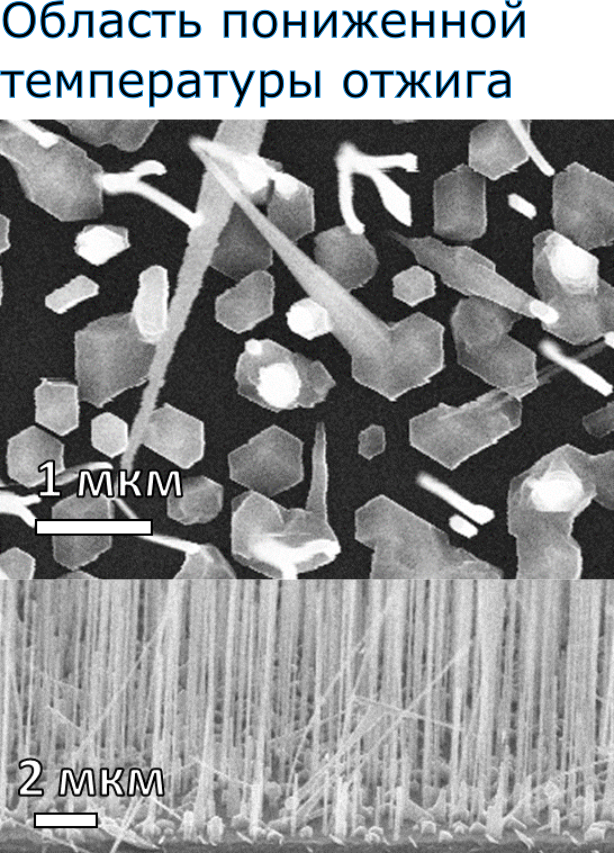
\includegraphics[width=0.27\linewidth]{Image_38_1}}
		\subcaptionbox{\label{fig:Image_38_2}}{%
		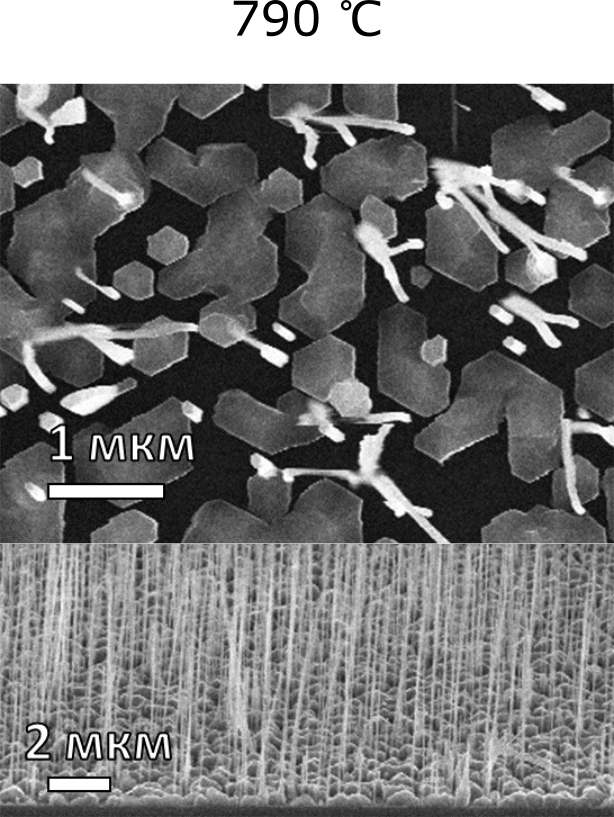
\includegraphics[width=0.27\linewidth]{Image_38_2}}
		\subcaptionbox{\label{fig:Image_38_3}}{%
		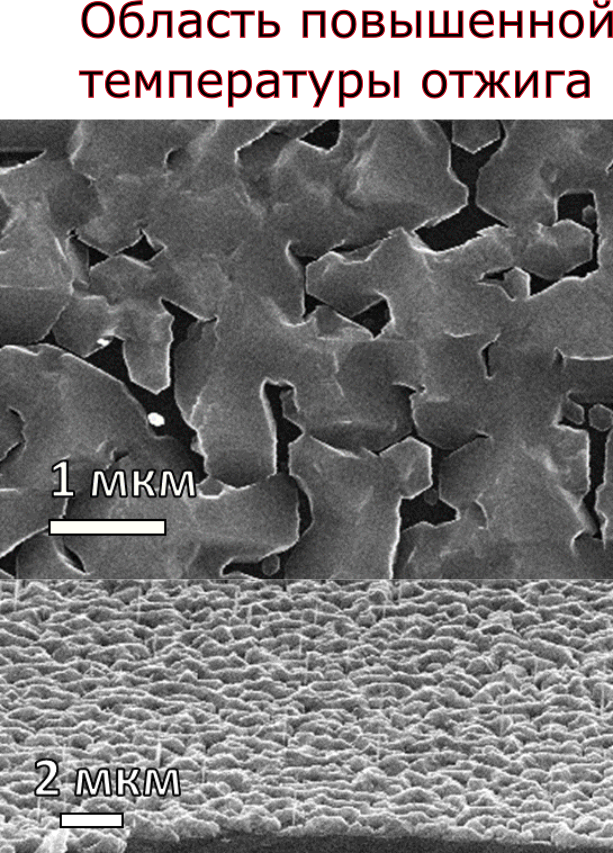
\includegraphics[width=0.27\linewidth]{Image_38_3}} } \caption{РЭМ
		изображения массивов ННК GaP, синтезированных на поверхности
		SiO\textsubscript{x}/Si(111), которая была отожжена при различной
температуре}\label{fig:Image_38} \end{figure}

В промежуточном случае (см.~рис.~\cref{fig:Image_38_2}) образуется плотный
вертикальный массив ННК. Известно, что отжиг вызывает частичную десорбцию
поверхностного SiO\textsubscript{x}, из-за чего снижается смачивание
поверхности каплями Ga, Можно предположить, что это смещает краевой угол
смачивания (краевой угол) в оптимальный диапазон для зарождения плотных
вертикальных ННК в режиме ПЖК \cite{Matteini2015}.

Метод подготовки поверхностного SiO\textsubscript{x} влияет на толщину, состав,
стойкость к химическому взаимодействию с Ga, температуру сгона оксида,
концентрацию поверхностных дефектов и поверхностную энергию, а следовательно
определяет оптимальную температуру отжига для получения максимальной плотности
и вертикальности массива ННК. Например для удаления поверхностного
SiO\textsubscript{x}, сформированного в азеотропном растворе
HNO\textsubscript{3}:H\textsubscript{2}O, потребовалось 30~\si{\minute} отжига
при температуре подложки выше 820~\si{\degreeCelsius}, тогда как поверхностный
SiO\textsubscript{x}, сформированный в 1:1:3 растворе
H\textsubscript{2}O\textsubscript{2}:NH\textsubscript{4}OH:H\textsubscript{2}O,
разлагается уже при 780~\si{\degreeCelsius}, что указывает на малую толщину и
более высокую степень отклонения его состава от стехиометрического
(см.~рис.~\cref{fig:Image_39}).

\begin{figure}[ht] \centerfloat{ \subcaptionbox{\label{fig:Image_39_1}}{%
		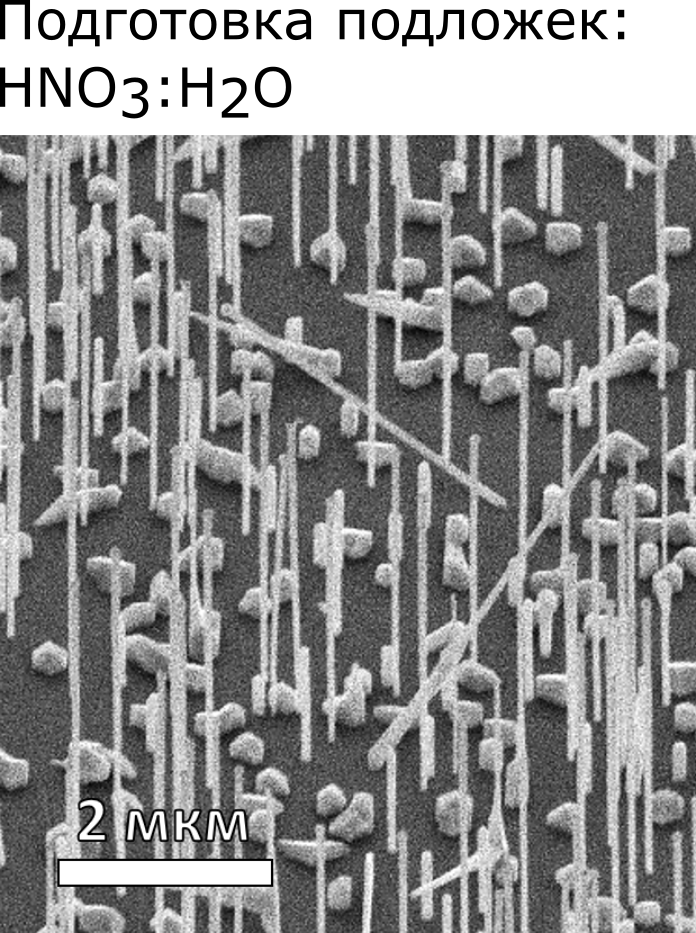
\includegraphics[width=0.23\linewidth]{Image_39_1}}
		\subcaptionbox{\label{fig:Image_39_2}}{%
		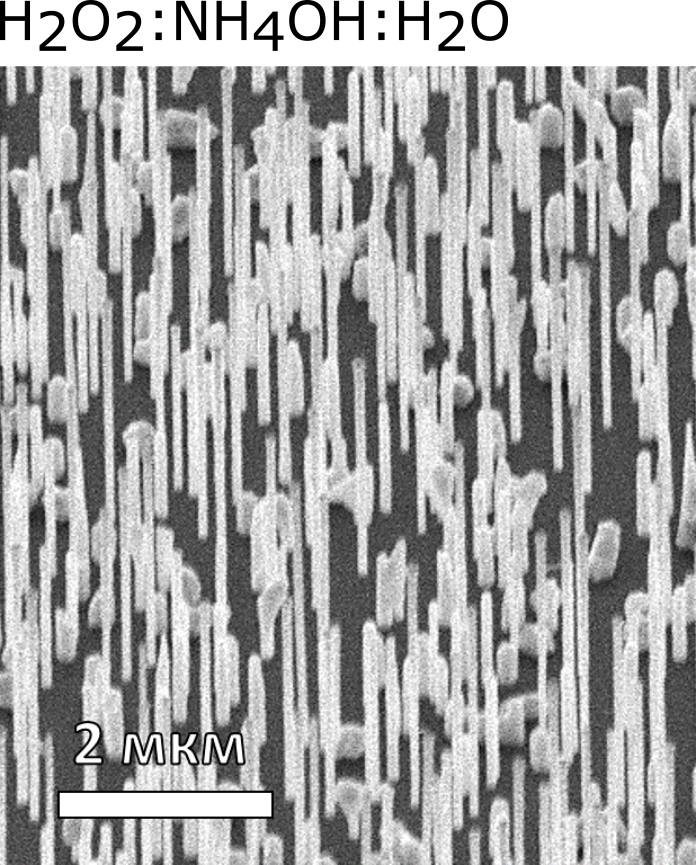
\includegraphics[width=0.23\linewidth]{Image_39_2}}

		\subcaptionbox{\label{fig:Image_39_3}}{%
		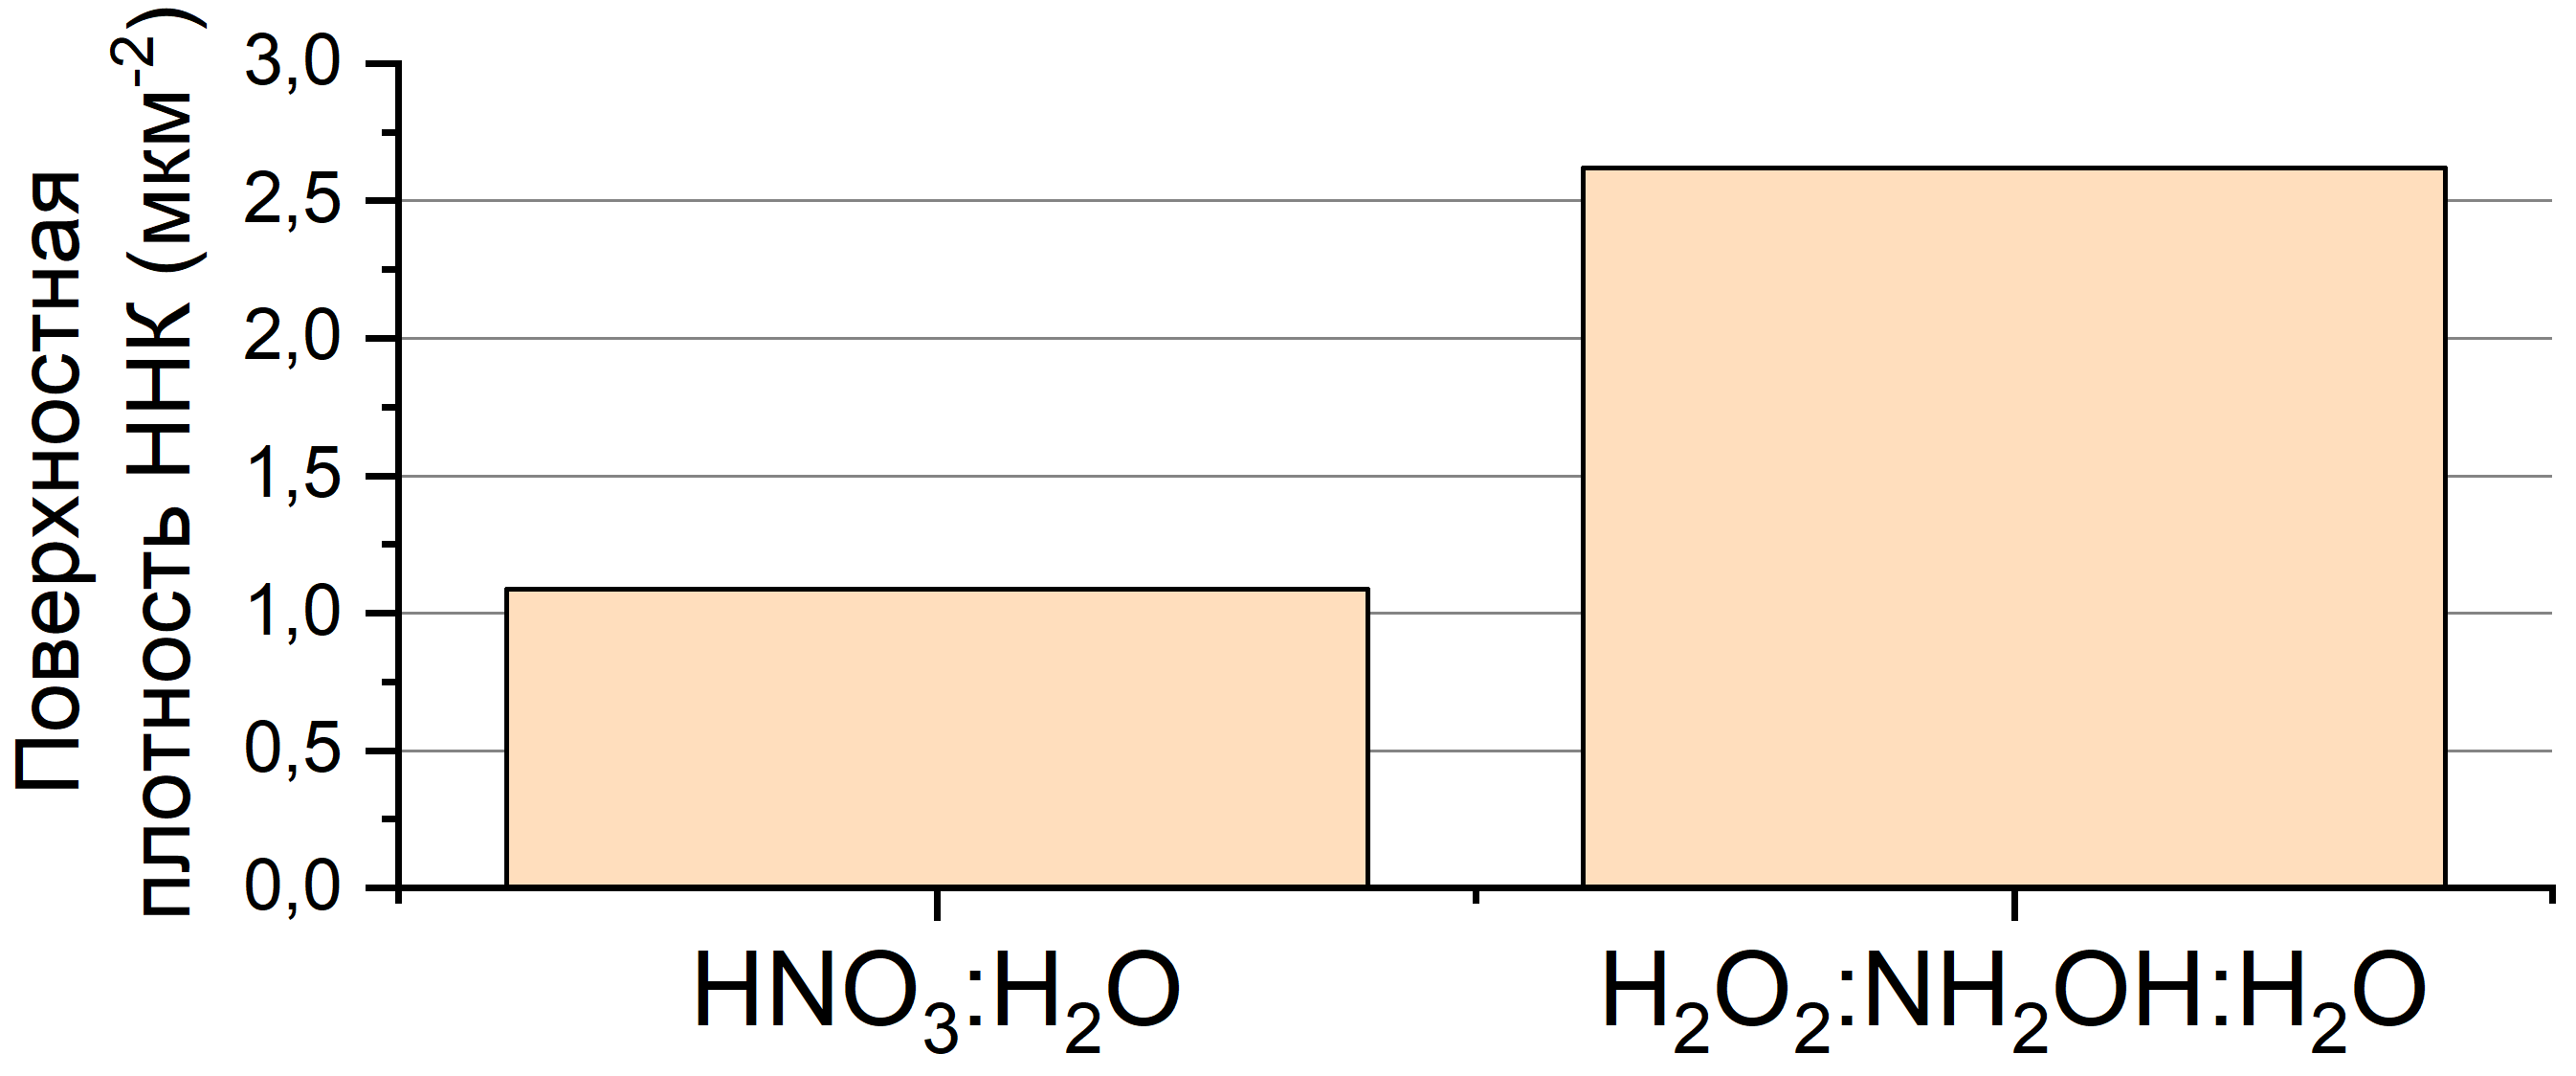
\includegraphics[width=0.6\linewidth]{Image_39_3}} } \caption{РЭМ
		изображения массивов ННК GaP (вид под углом 30{\textdegree}),
		выращенных на поверхностном SiO\textsubscript{x}, подготовленном в
		азеотропном растворе HNO\textsubscript{3}:H\textsubscript{2}O~(а) и в
		кипящем растворе
		H\textsubscript{2}O\textsubscript{2}:NH\textsubscript{2}OH:H\textsubscript{2}O~(б),
	сравнение поверхностных плотностей массивов ННК~(в)}\label{fig:Image_39}
\end{figure}

Для сравнения влияния метода подготовки оксида, подложки отжигались при
температуре на 30~\si{\degreeCelsius} ниже температуры быстрого сгона с целью
изучить формирование плотных вертикальных массив ННК. По сравнению с оксидом,
подготовленным в кипящем азеотропном растворе
HNO\textsubscript{3}:H\textsubscript{2}O, оксид, сформированный в кипящем
растворе
H\textsubscript{2}O\textsubscript{2}:NH\textsubscript{4}OH:H\textsubscript{2}O
приводит к образованию массива с плотностью вертикальных ННК в 2,5 раза выше,
меньшей концентрацией наклонных ННК и островков (см.~рис.~\cref{fig:Image_39}).
Поэтому в следующих экспериментах оксид подготавливался в кипящем растворе
H\textsubscript{2}O\textsubscript{2}:NH\textsubscript{4}OH:H\textsubscript{2}O
(температура кипения 80--85~\si{\degreeCelsius}).

Для формирования капель достаточного размера для зарождения ННК в некоторых
работах перед ростом на поверхность подложки дополнительно наносят Ga
\cite{Plissard2010}. Чтобы оценить его влияние выращено два образца при
аналогичных условиях роста (соотношение ЭДП P/Ga \(\approx 6\), что соответствует
стехиометрическому отношению адатомов на поверхности подложки; температура
роста 610~\si{\degreeCelsius}; время роста 5~\si{\minute}). Формирование
первого образца начиналось одновременным открытием заслонок Ga и P, а
второго~--- нанесением Ga эквивалентной толщиной 1~\si{\nano\meter}
(см.~рис.~\cref{fig:Image_40}).

\begin{figure}[ht] \centerfloat{ \subcaptionbox{\label{fig:Image_40_1}}{%
		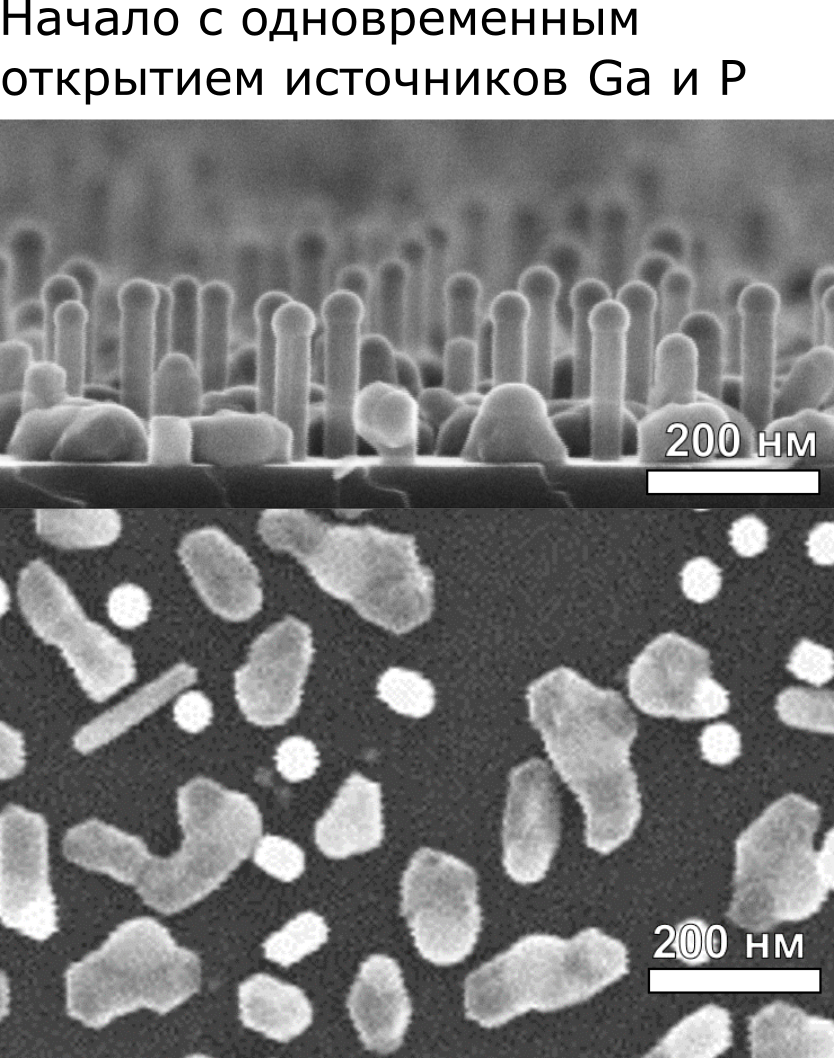
\includegraphics[width=0.4\linewidth]{Image_40_1}}
		\subcaptionbox{\label{fig:Image_40_2}}{%
		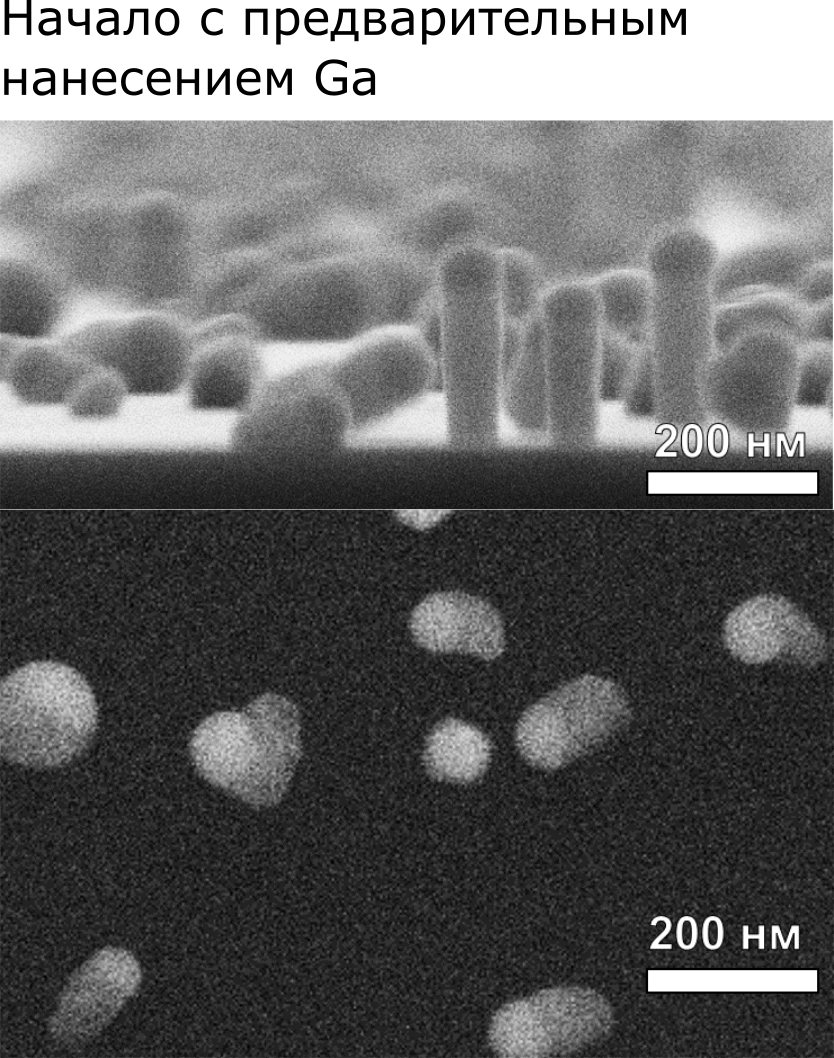
\includegraphics[width=0.4\linewidth]{Image_40_2}} } \caption{РЭМ
		изображения ННК GaP образца, выращенного при одновременном открытии
		источников Ga и P~(а), и образца, выращенного с предварительным
		нанесением Ga эквивалентной толщиной
1~{\si{\nano\metre}}~(б)}\label{fig:Image_40} \end{figure}

Из РЭМ изображений видно, что капли необходимой для зарождения ННК морфологии
(размера и краевого угла смачивания) могут формироваться в присутствии адатомов
P, при этом предварительное нанесение Ga ведёт к снижению плотности
вертикальных ННК.

\section{Изменение морфологии массива в процессе роста}\label{sec:ch5/sec3}

Рассматриваемые образцы
(см.~рис.~\cref{fig:Image_43_12},~\cref{fig:Image_43_34}) выращены с разной продолжительностью осаждения GaP при сохранении остальных параметров роста (температура
роста 630~\si{\degreeCelsius}; поток Ga в 1~отн.~ед.; соотношение ЭДП P/Ga~24).

Поверхностная плотность ННК увеличивается со временем роста, что указывает на растянутую во времени стадию зарождения (см.~рис.~\cref{fig:Image_43_3}).
Длина ННК линейно со временем увеличивается со скоростью
80~\si{\nano\meter\per\minute} (см.~рис.~\cref{fig:Image_43_1}). При этом
наблюдается изменение формы ННК: сужение к основанию переходит в сужение к
вершине (см.~рис.~\cref{fig:Image_43_2}) из-за стабилизация верхнего диаметра. Данный эффект может быть объяснен существованием равновесного диаметра капли катализатора, при
котором потоки поступающих в каплю адатомов Ga и P выравниваются, а увеличение
основания~--- боковым ростом в режиме пар\,--\,кристалл.

\begin{figure}[ht]
	\centerfloat{
		\subcaptionbox{\label{fig:Image_43_1}}{%
		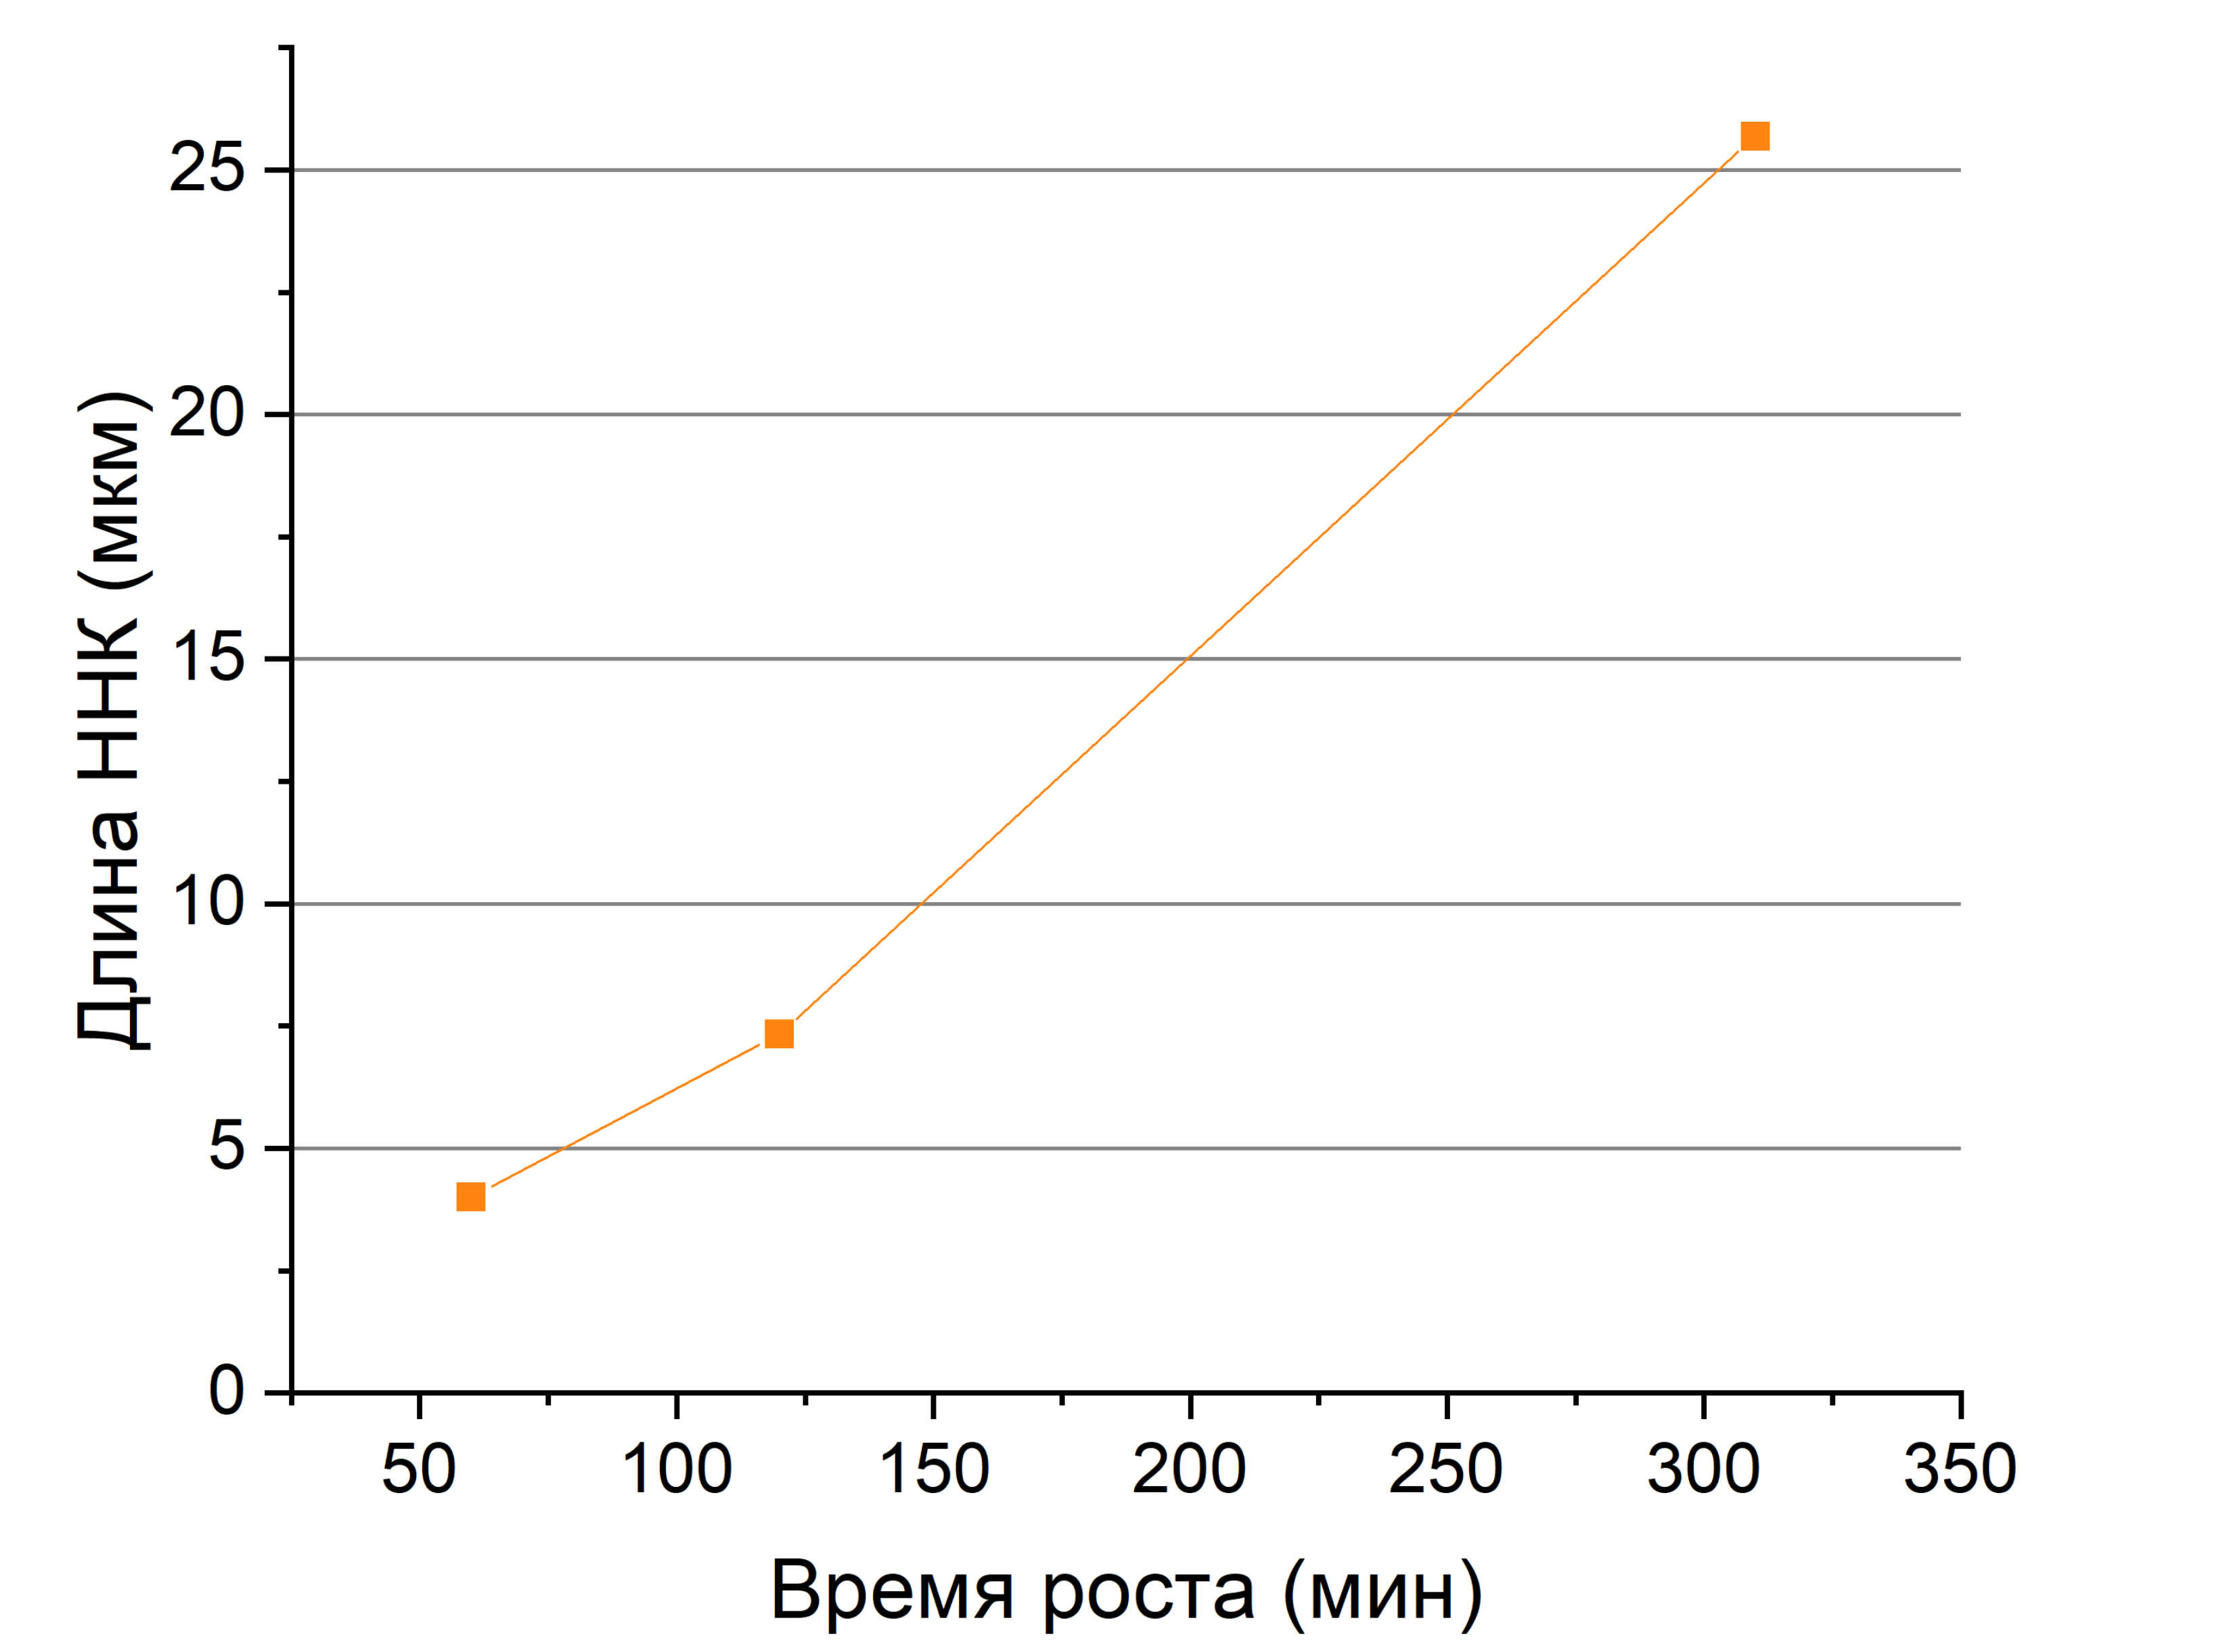
\includegraphics[width=0.48\linewidth]{Image_43_1}}
		\subcaptionbox{\label{fig:Image_43_2}}{%
	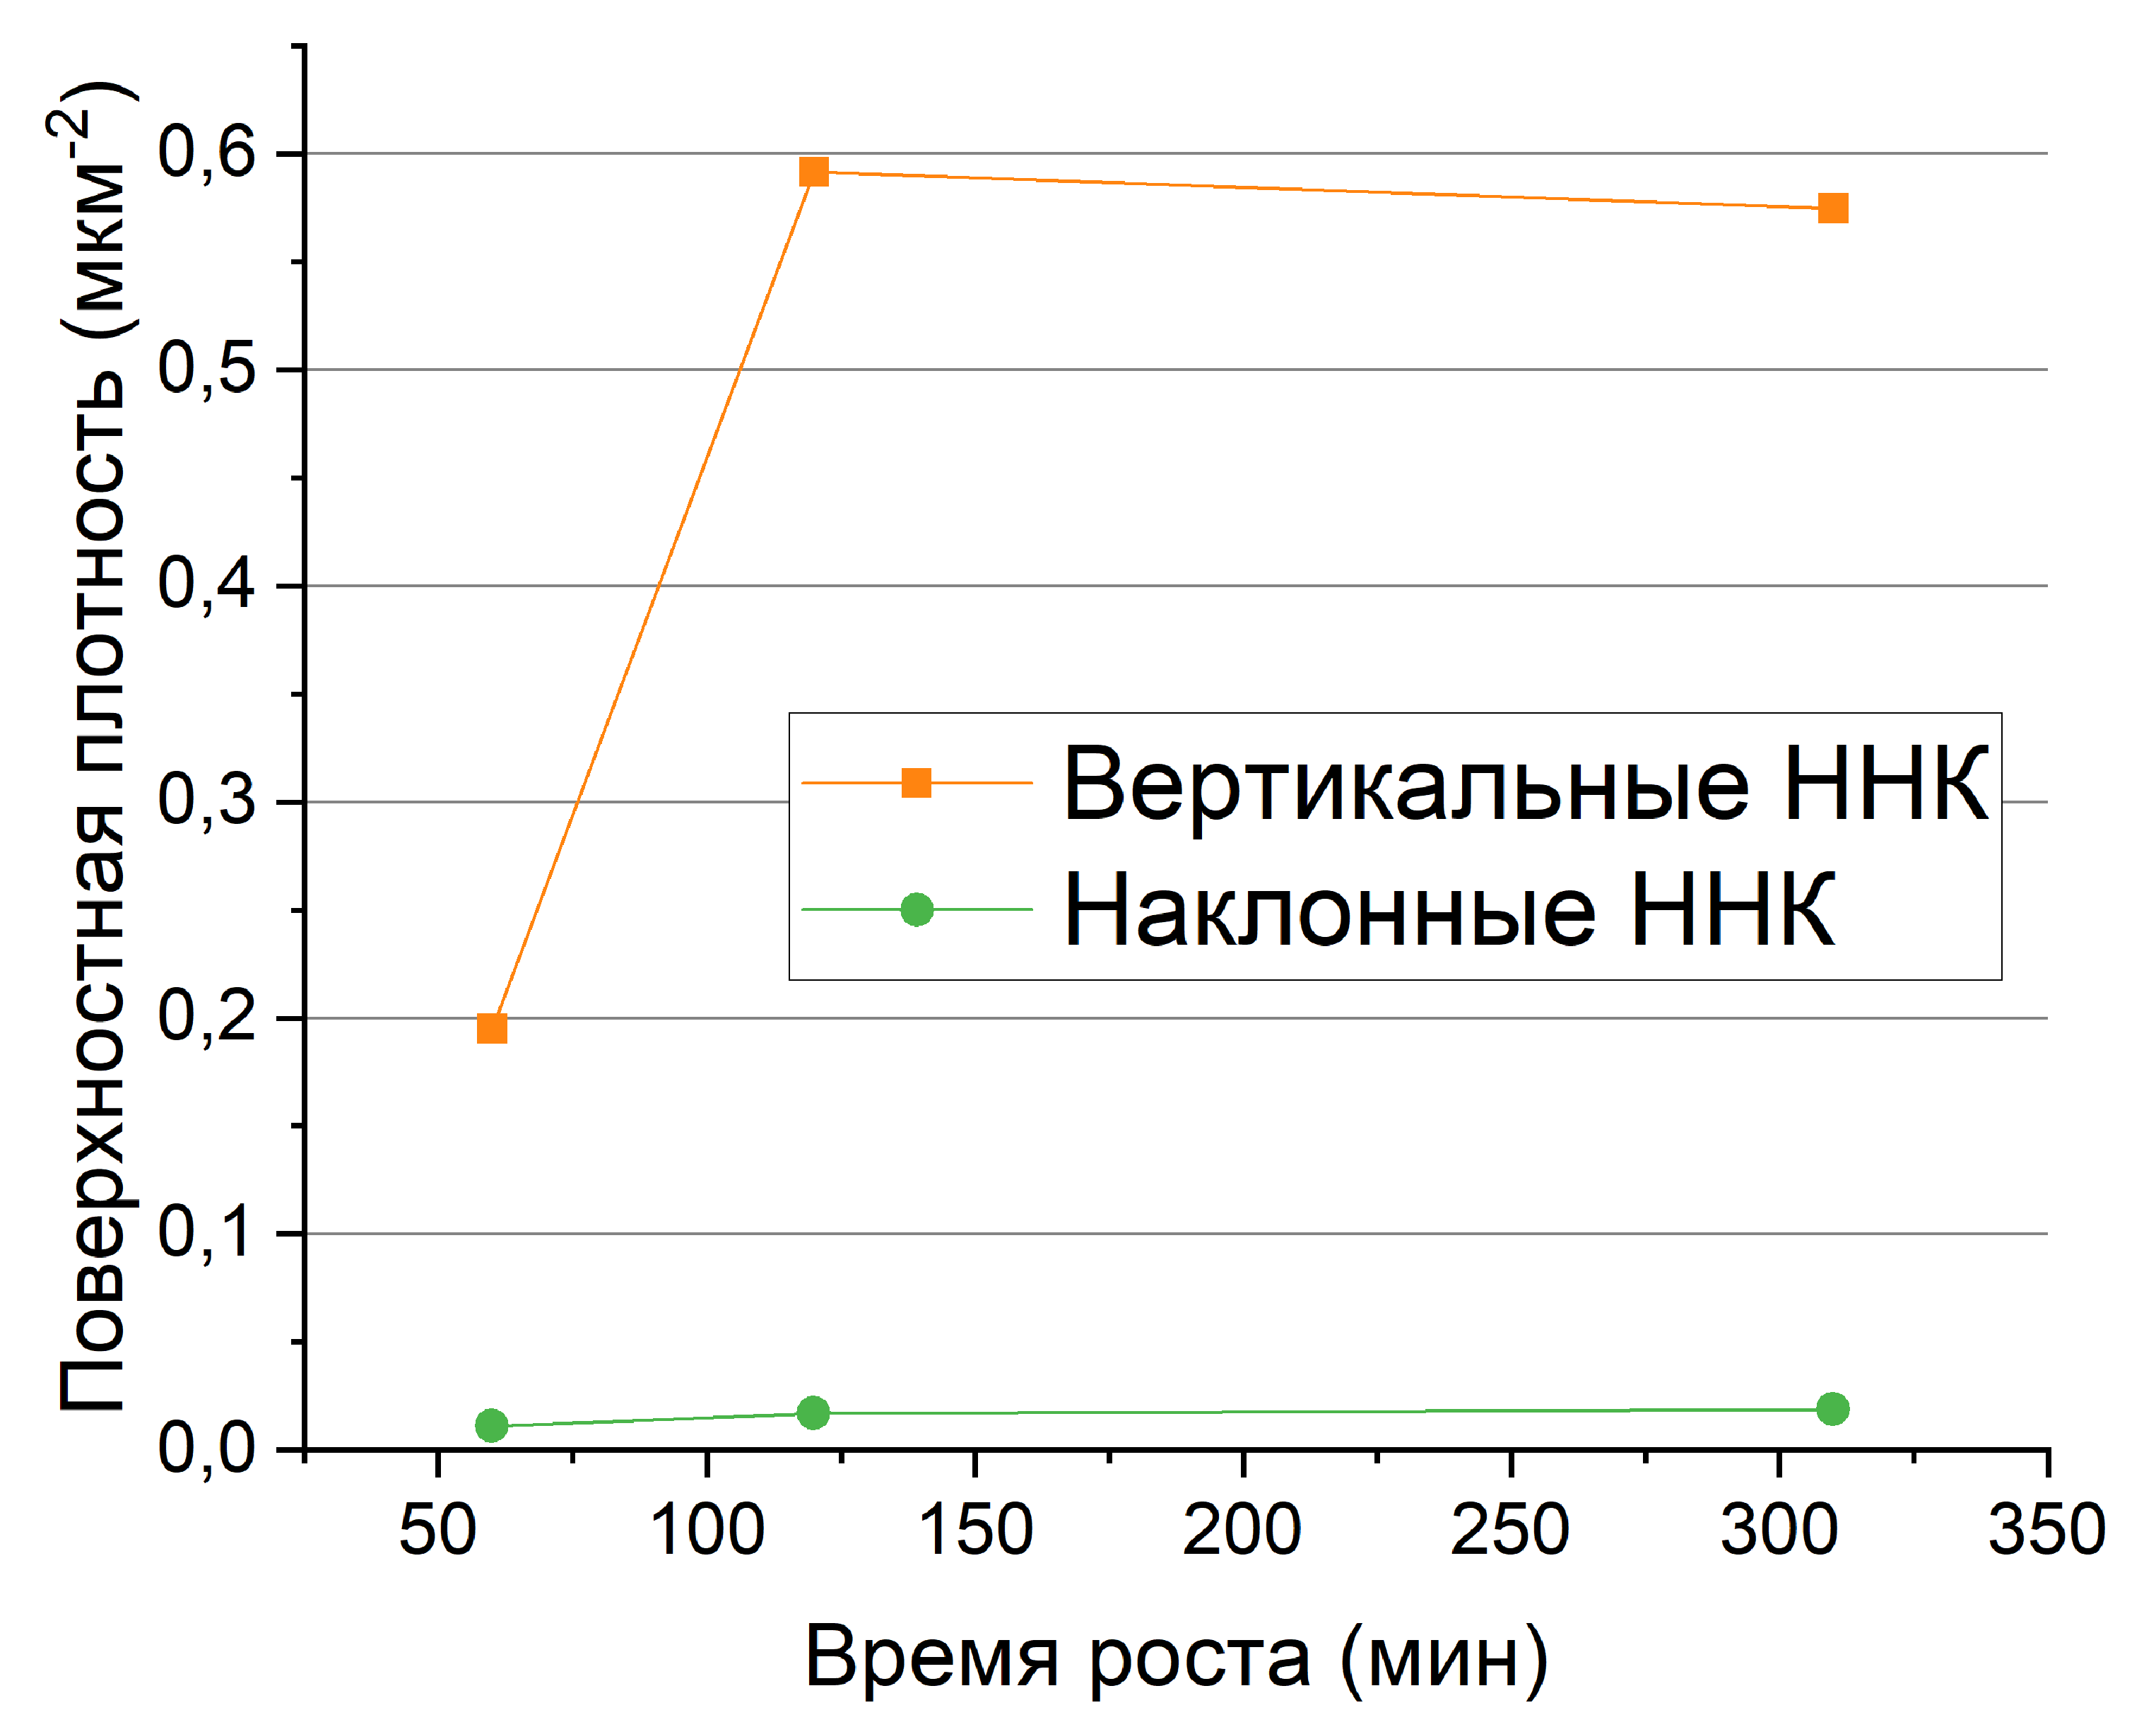
\includegraphics[width=0.48\linewidth]{Image_43_2}}
}
\caption{График изменения длин~(а) и диаметров вершин~(б) ННК GaP в процессе роста}
\label{fig:Image_43_12}
\end{figure}

\begin{figure}[ht]
	\centerfloat{
		\subcaptionbox{\label{fig:Image_43_3}}{%
		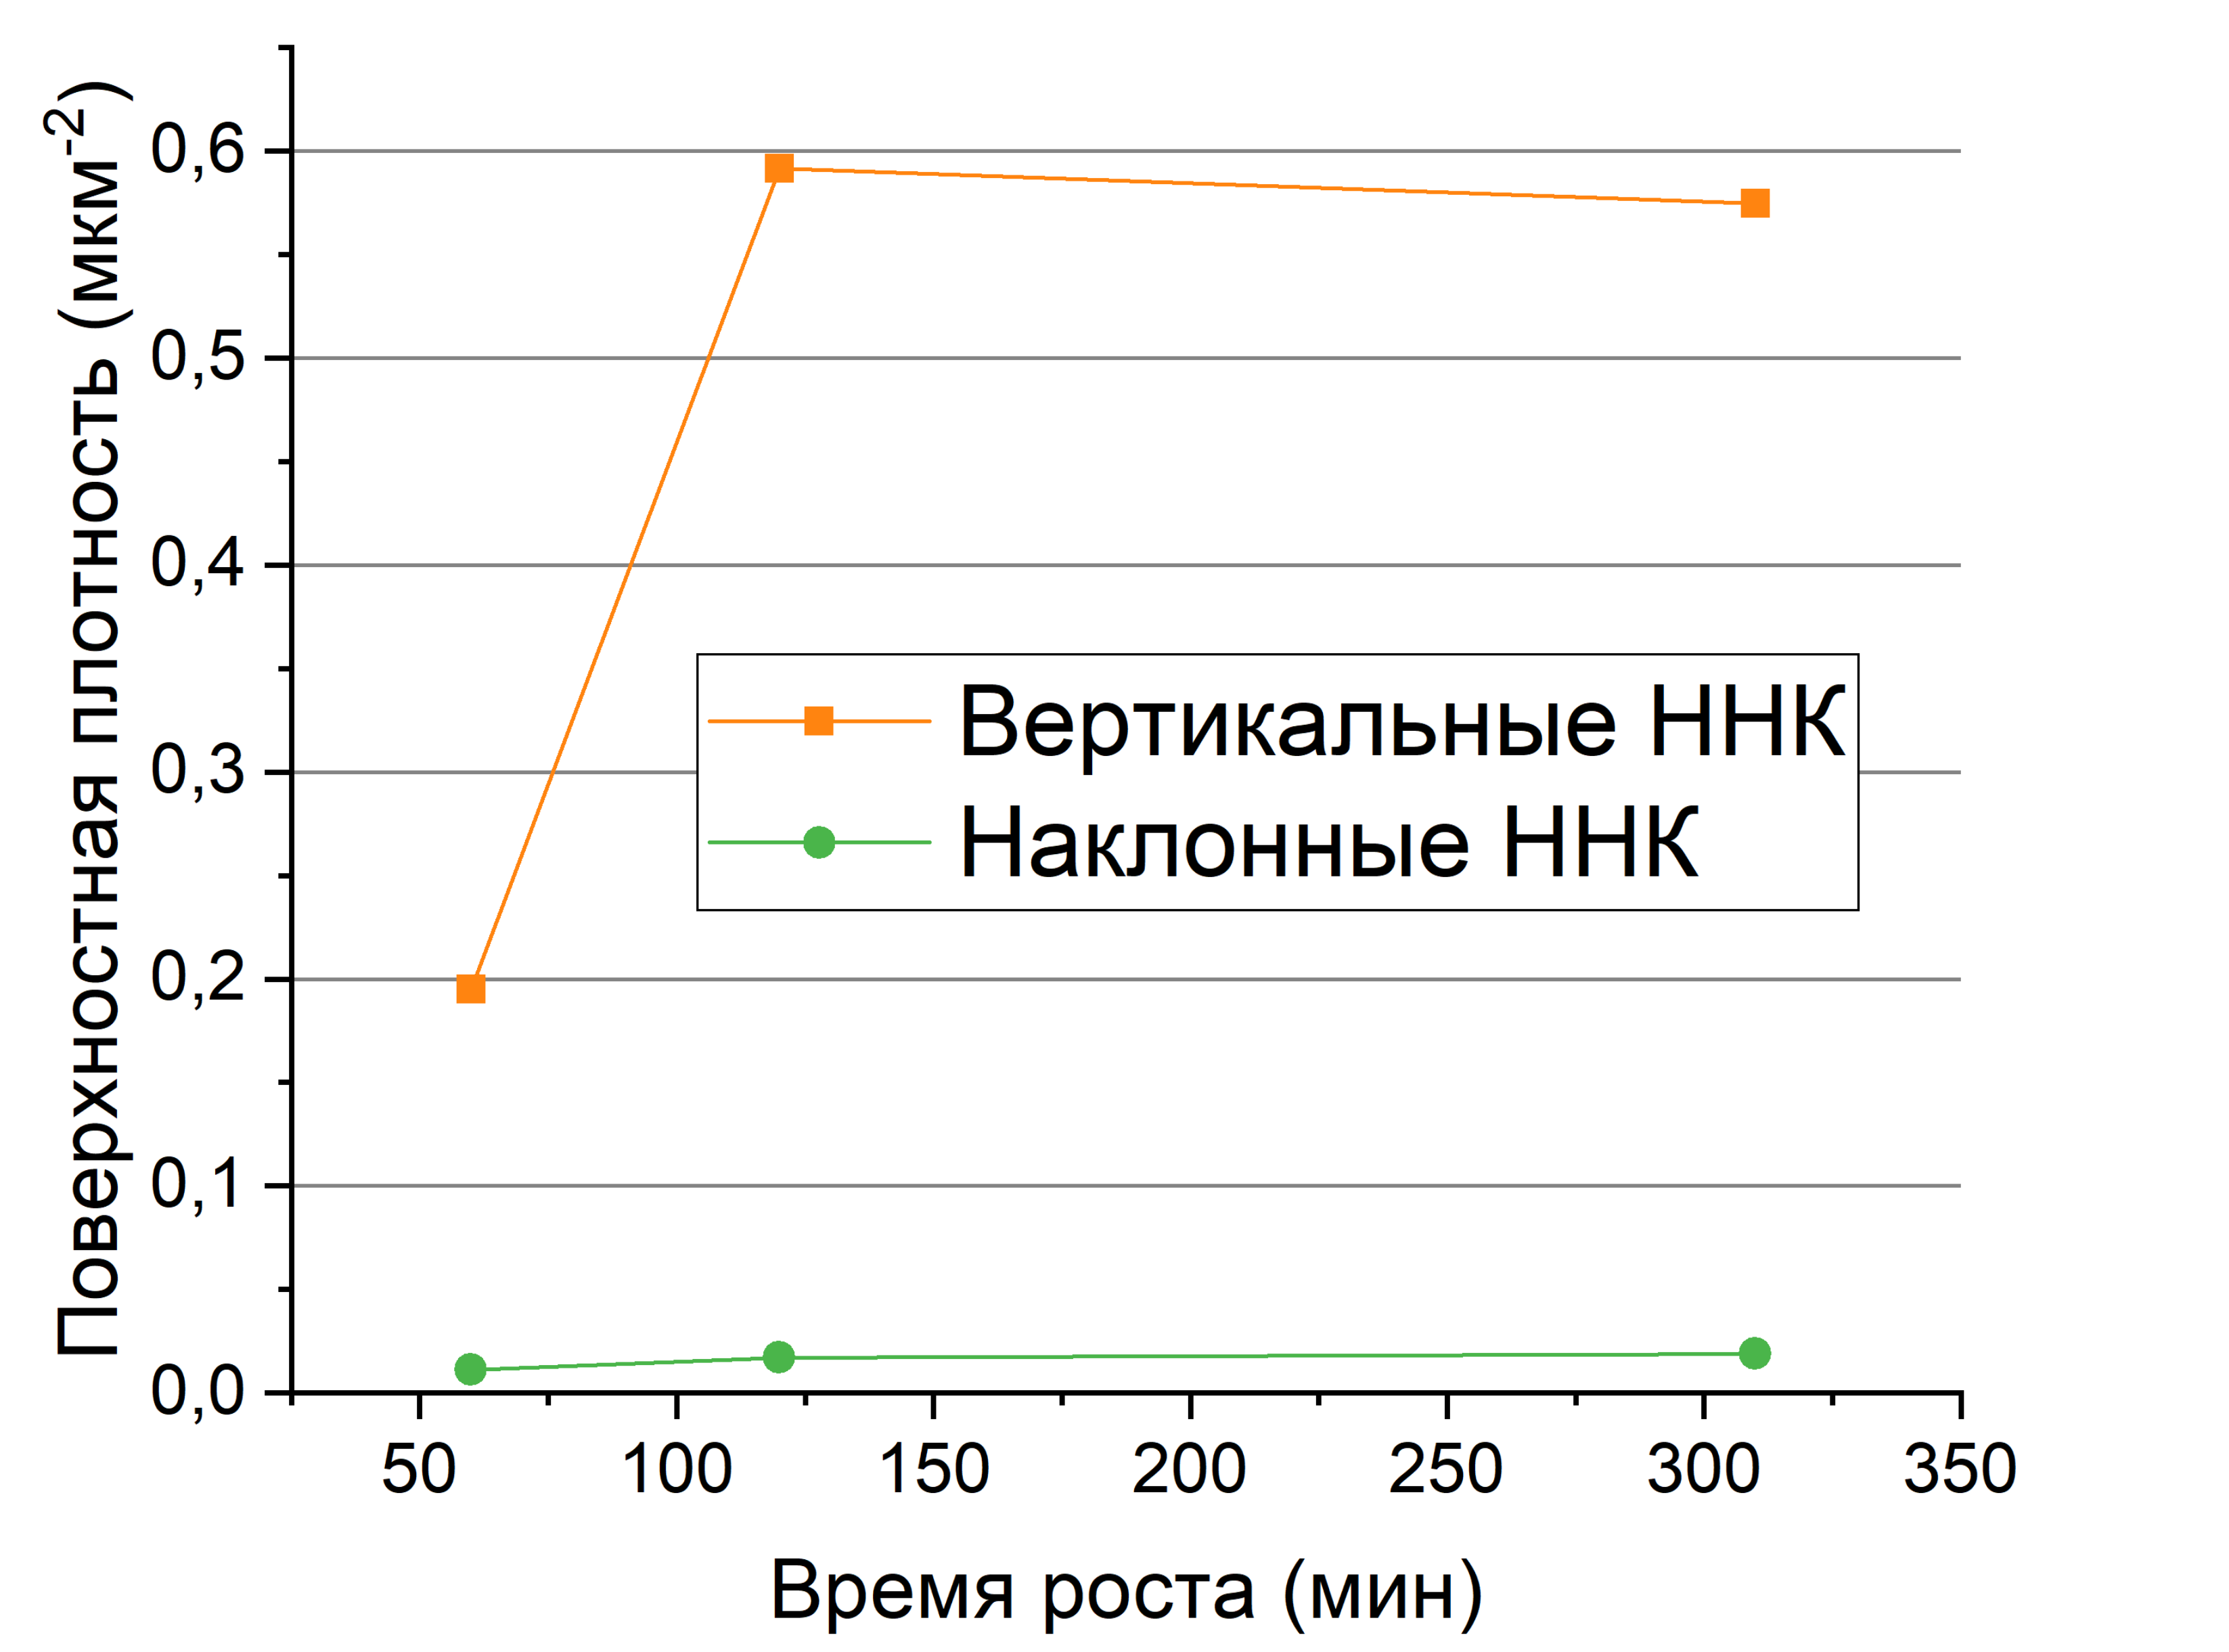
\includegraphics[width=0.48\linewidth]{Image_43_3}}
		\subcaptionbox{\label{fig:Image_43_4}}{%
		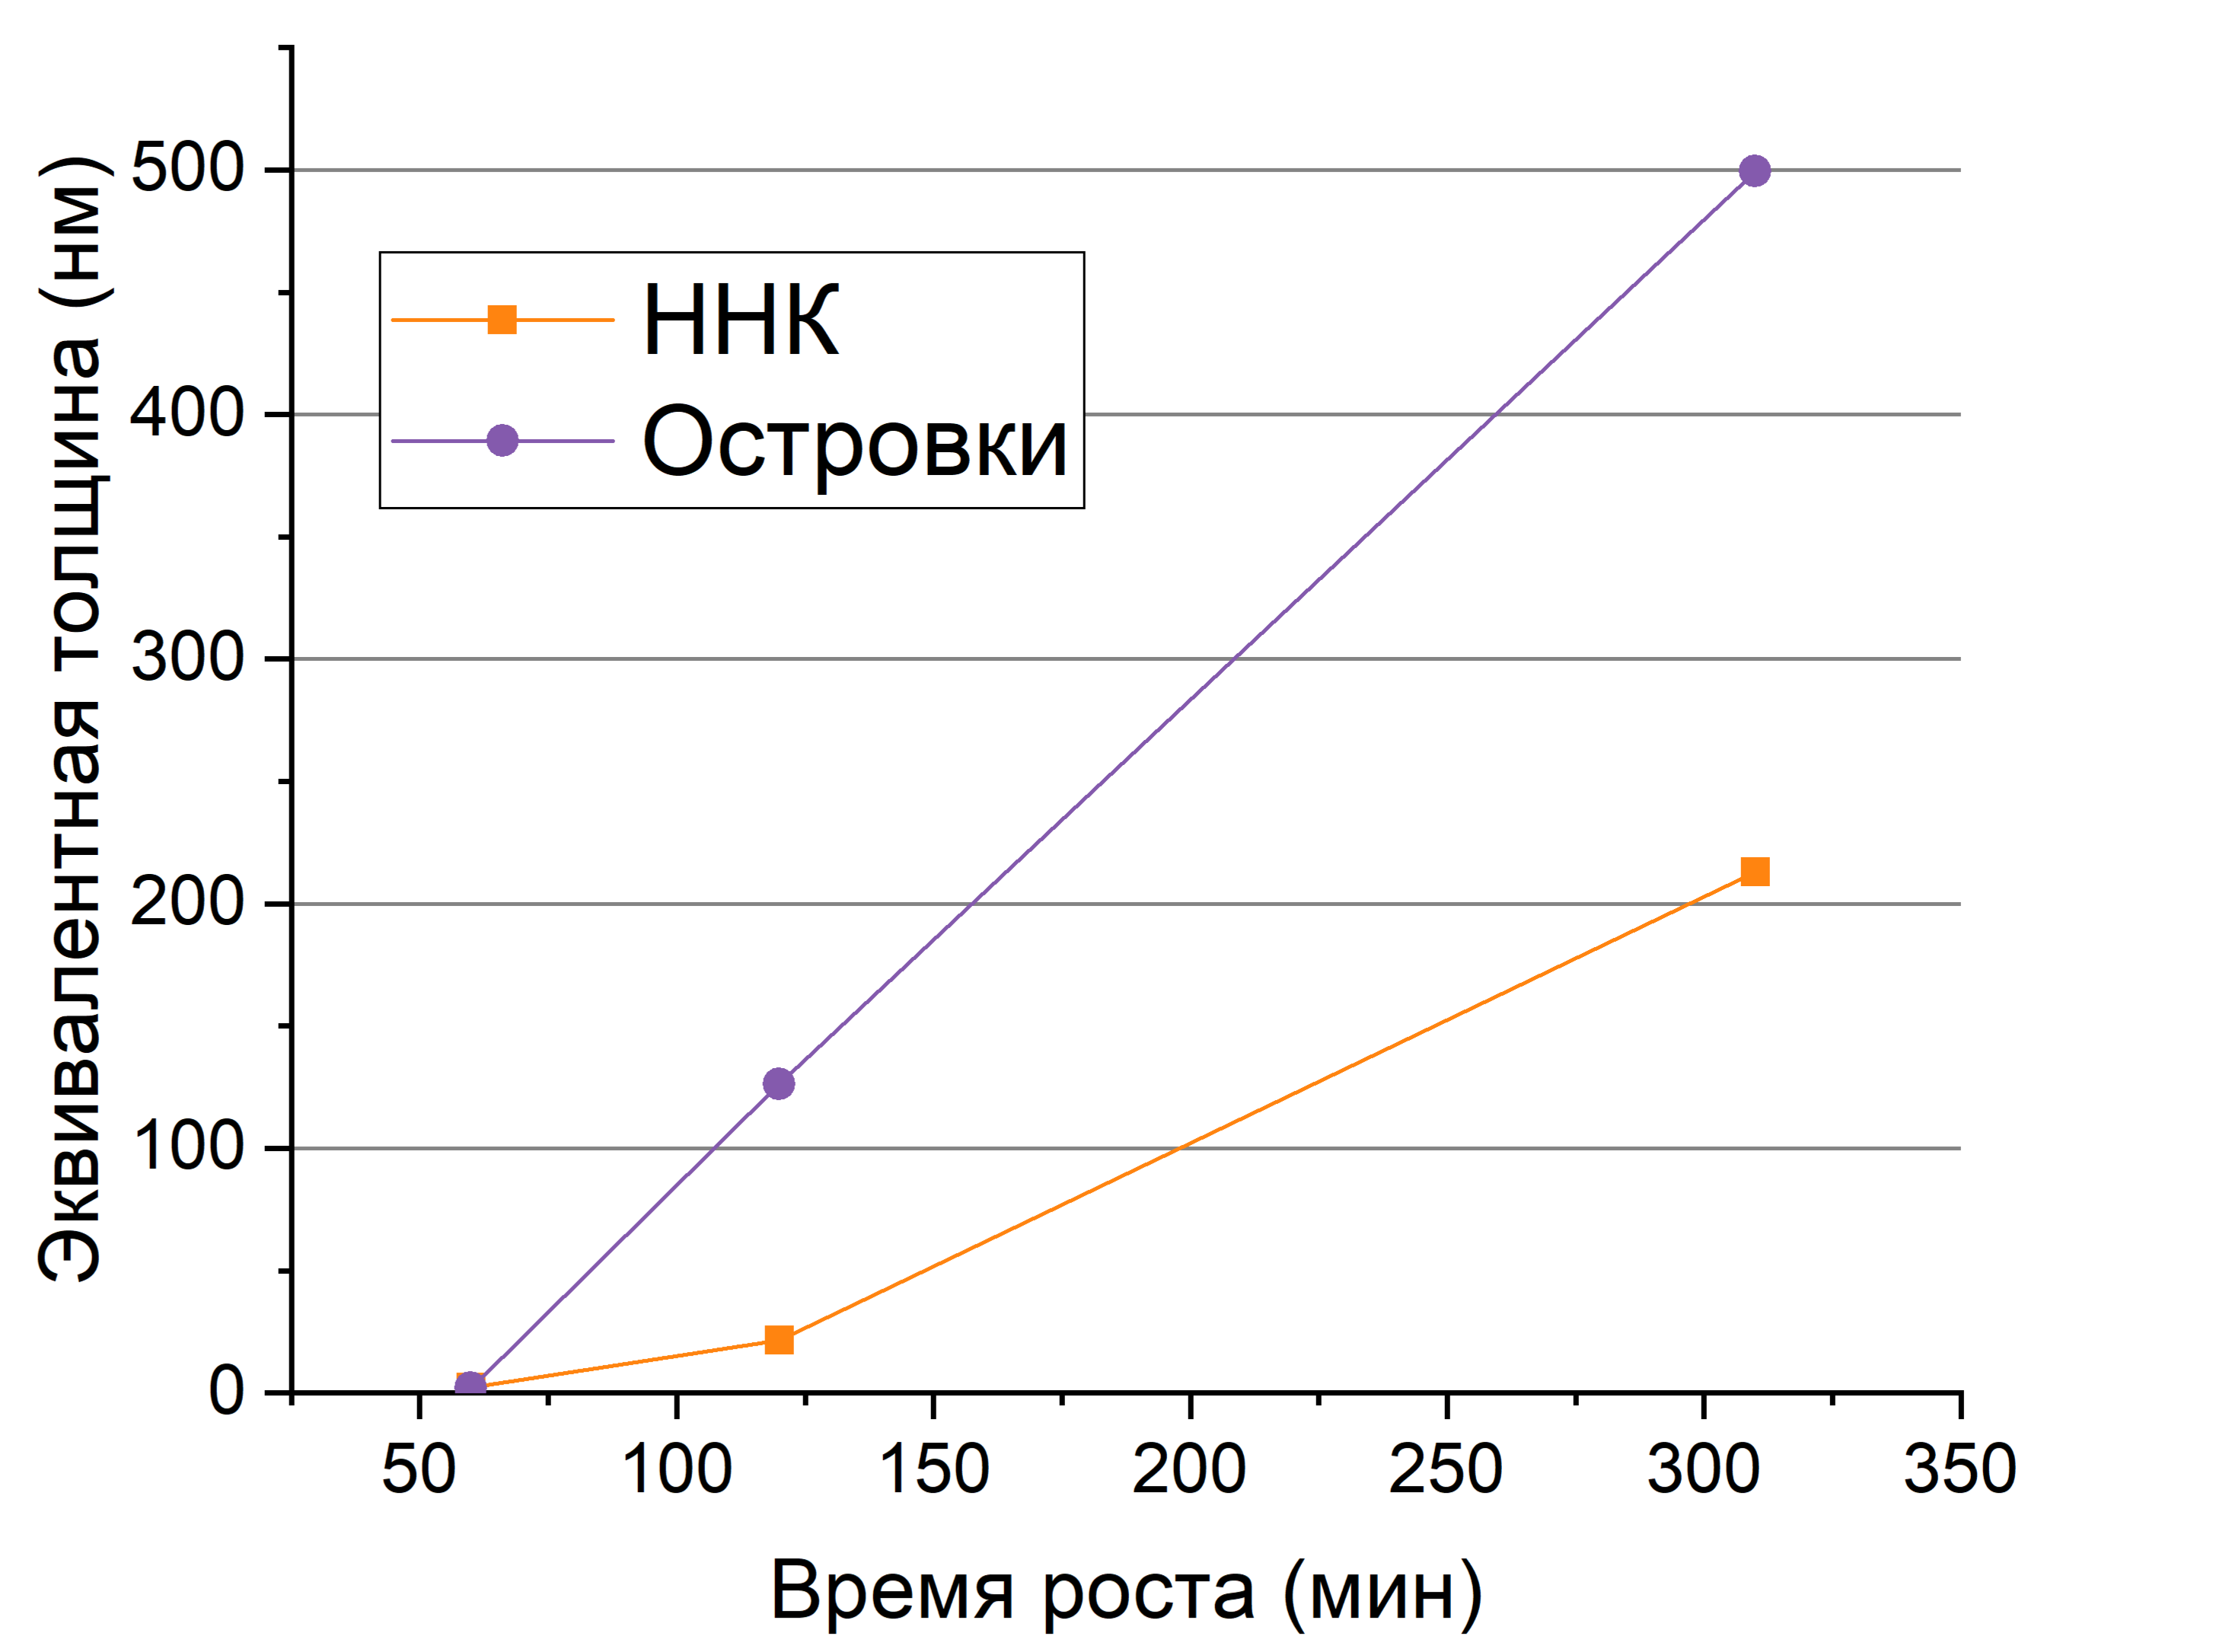
\includegraphics[width=0.48\linewidth]{Image_43_4}}
}
\caption{График изменения поверхностной плотности~(б) и эквивалентной толщины~(в) массива ННК
GaP в процессе роста}
\label{fig:Image_43_34}
\end{figure}

В случае ПЖК роста размер вершины ННК пропорционален размеру капли катализатора
\cite{glas2010vapor}, которая почти полностью состоит из Ga в случае роста GaP
или GaAs. Изменение объёма капли \(V\) контролируется скоростью кристаллизации
\(dL/dt\) и величиной потока атомов Ga в каплю. Последняя определяется прямым
попаданием атомов из молекулярного потока и диффузионным потоком адатомов по
боковым стенкам ННК к капле \cite{glas2010vapor}. Таким образом изменение объема капли со временем определяется следующим выражением:

\begin{equation} \label{eq:equation1} \frac{dV}{dt}=D_{top}^2 \frac{\pi F_{Ga}
	f(\theta,\phi)}{4}+ D_{top} F_{Ga} \lambda \tan{\phi} - D_{top}^2 \frac{dL}{dt}
	\frac{\pi}{4},
\end{equation}
где \(F_{Ga}\)~--- поток Ga~(\si{\nano\meter\per\second}),
\(f(\theta,\phi)\)~--- геометрический фактор, который является функцией
контактного угла капли (\(\theta\)) и угла падения молекулярного пучка
(\(\phi\)) \cite{glas2010vapor}, \(\lambda\)~--- длина свободного пробега
адатомов Ga на боковых стенках ННК.

При стабильном краевом угле (\(\theta\)) объем капли можно рассчитать по следующей формуле: 

\begin{equation}
	\label{eq:equation7} V=\frac{g(\theta,\phi)D_{top}^3}{12},
\end{equation}
где \(g(\theta,\phi)\)~--- геометрический фактор.

С учётом уравнения~\ref{eq:equation1}, эволюция радиуса вершины ННК описывается
уравнением:

\begin{equation} \label{eq:equation2} g(\theta) \frac{dD_{top}}{dt}=F_{Ga}
	f(\theta,\phi)+ F_{Ga} \frac{4 \lambda}{\pi D_{top}} \tan{\phi}-\frac{dL}{dt}.
\end{equation}

В самокаталитическом процессе скорость осевого роста ограничена потоком атомов
V группы к капле \(F_P\), который поддерживался постоянным в рассматриваемой
экспериментальной серии.

В работах
\cite{tersoff2015stable,dubrovskii2016regimes,berdnikov2020comparison} показали
стабилизацию размеров Ga капель в массивах GaAs ННК. В данном эксперименте наблюдается подобный эффект для GaP
ННК. Условие стабилизации объёма и верхнего
радиуса (\(D_{top} = D_{top}^\ast = const\)) требует выполнения условия
\(dD_{top} / dt = 0\). Таким образом, с учётом уравнения~\ref{eq:equation2}
можно вывести выражения для стабильного
диаметра~(см.~уравнение~\ref{eq:equation3}) и осевой скорости роста
ННК~(см.~уравнение~\ref{eq:equation4}):

\begin{equation} \label{eq:equation3}
D_{top}^\ast=\frac{4 \lambda \tan{\phi}}{\pi f(\theta,\phi)(\frac{F_{P}}{F_{Ga}} - 1)};
\end{equation}

\begin{equation} \label{eq:equation4} \frac{dL}{dt}=F_{Ga} \left(
	f(\theta,\phi) + \frac{4 \lambda}{\pi D_{top}^\ast}\tan{\phi} \right)=const.
\end{equation}

Если пренебречь нелинейностью скорости роста на начальном этапе роста, то длина ННК задаётся
уравнением~\ref{eq:equation5}:

\begin{equation} \label{eq:equation5} L\approx F_{Ga} \Delta t \left(
	f(\theta,\phi) + \frac{4 \lambda \tan{\phi}}{\pi D_{top}^\ast} \right).
\end{equation}

Зная \(F_ {Ga}\) и \(f(\theta,\phi)\) при экспериментально определённых
\(\theta = 120\si{\degree}\) и \(\phi = 34\si{\degree}\), можно использовать
наклон временной зависимости \(L(t)\) в уравнении~\ref{eq:equation5}, чтобы
оценить \(\lambda\):

\begin{equation} \label{eq:equation6} \lambda=D_{top}^\ast
	\frac{\pi}{4\tan{\phi}} \left( \frac{L}{\Delta t F_{Ga}}-f(\theta,\phi)
\right).  \end{equation}

Уравнение~\ref{eq:equation6} даёт оценку для \(\lambda\) исходя из
экспериментально наблюдаемых значений.

\section{Влияние отношения ЭДП P/Ga}\label{sec:ch5/sec4}

%[10.1088/0957-4484/21/38/385602] These observations can be fully explained by
%a Ga droplet-assisted VLS mechanism [12, 13, 31]. When group V flow is too
%low, Ga accumulates in the particle over time, leading to a diameter
%expansion, and as the droplet defines the threephase boundary at which
%nanowire growth occurs [38, 39], nanowire diameter increases as well. A
%slightly higher group V flux leads to a dynamical steady state, where constant
%Ga droplet size is maintained over the nanowire length. But if group V becomes
%too high, the Ga droplet shrinks over time and tapering occurs. Some lateral
%growth via a vapor- solid mechanism (direct incorporation on the sidewalls)
%cannot be ruled out and could also contribute to the tapering, as a high group
%V flux reduces group III adatom mobility on the sidewalls. If very high As
%flux is used (d), the Ga droplet is rapidly consumed and the VLS process is
%terminated, in favor of 2D bulk growth, as observed here.

Исследуемые образцы синтезировались при соотношении ЭДП P/Ga \(\approx
12/18/24/30\), постоянном времени роста (1~\si{\hour}), потоке Ga в 2~отн.~ед.
Рост ННК начинался одновременным открытием заслонок источников Ga и P при
температуре подложки T\textsubscript{роста} \(\approx
610\)~\si{\degreeCelsius}.

Увеличение отношения ЭДП P/Ga с 12 до 24 приводит к увеличению длины и
уменьшению диаметра ННК (см.~рис.~\cref{fig:Image_41_1}). Последний эффект
может быть объяснён уменьшением стабильного диаметра капли, при котором
выравниваются потоки атомов P и Ga, попадающих в каплю. Увеличение ЭДП P/Ga до
30 привело к полному поглощению капли, что, в свою очередь, привело к остановке
осевого роста в режиме ПЖК и продолжении роста в режиме пар\,--\,кристалл.

\begin{figure}[ht] \centerfloat{
		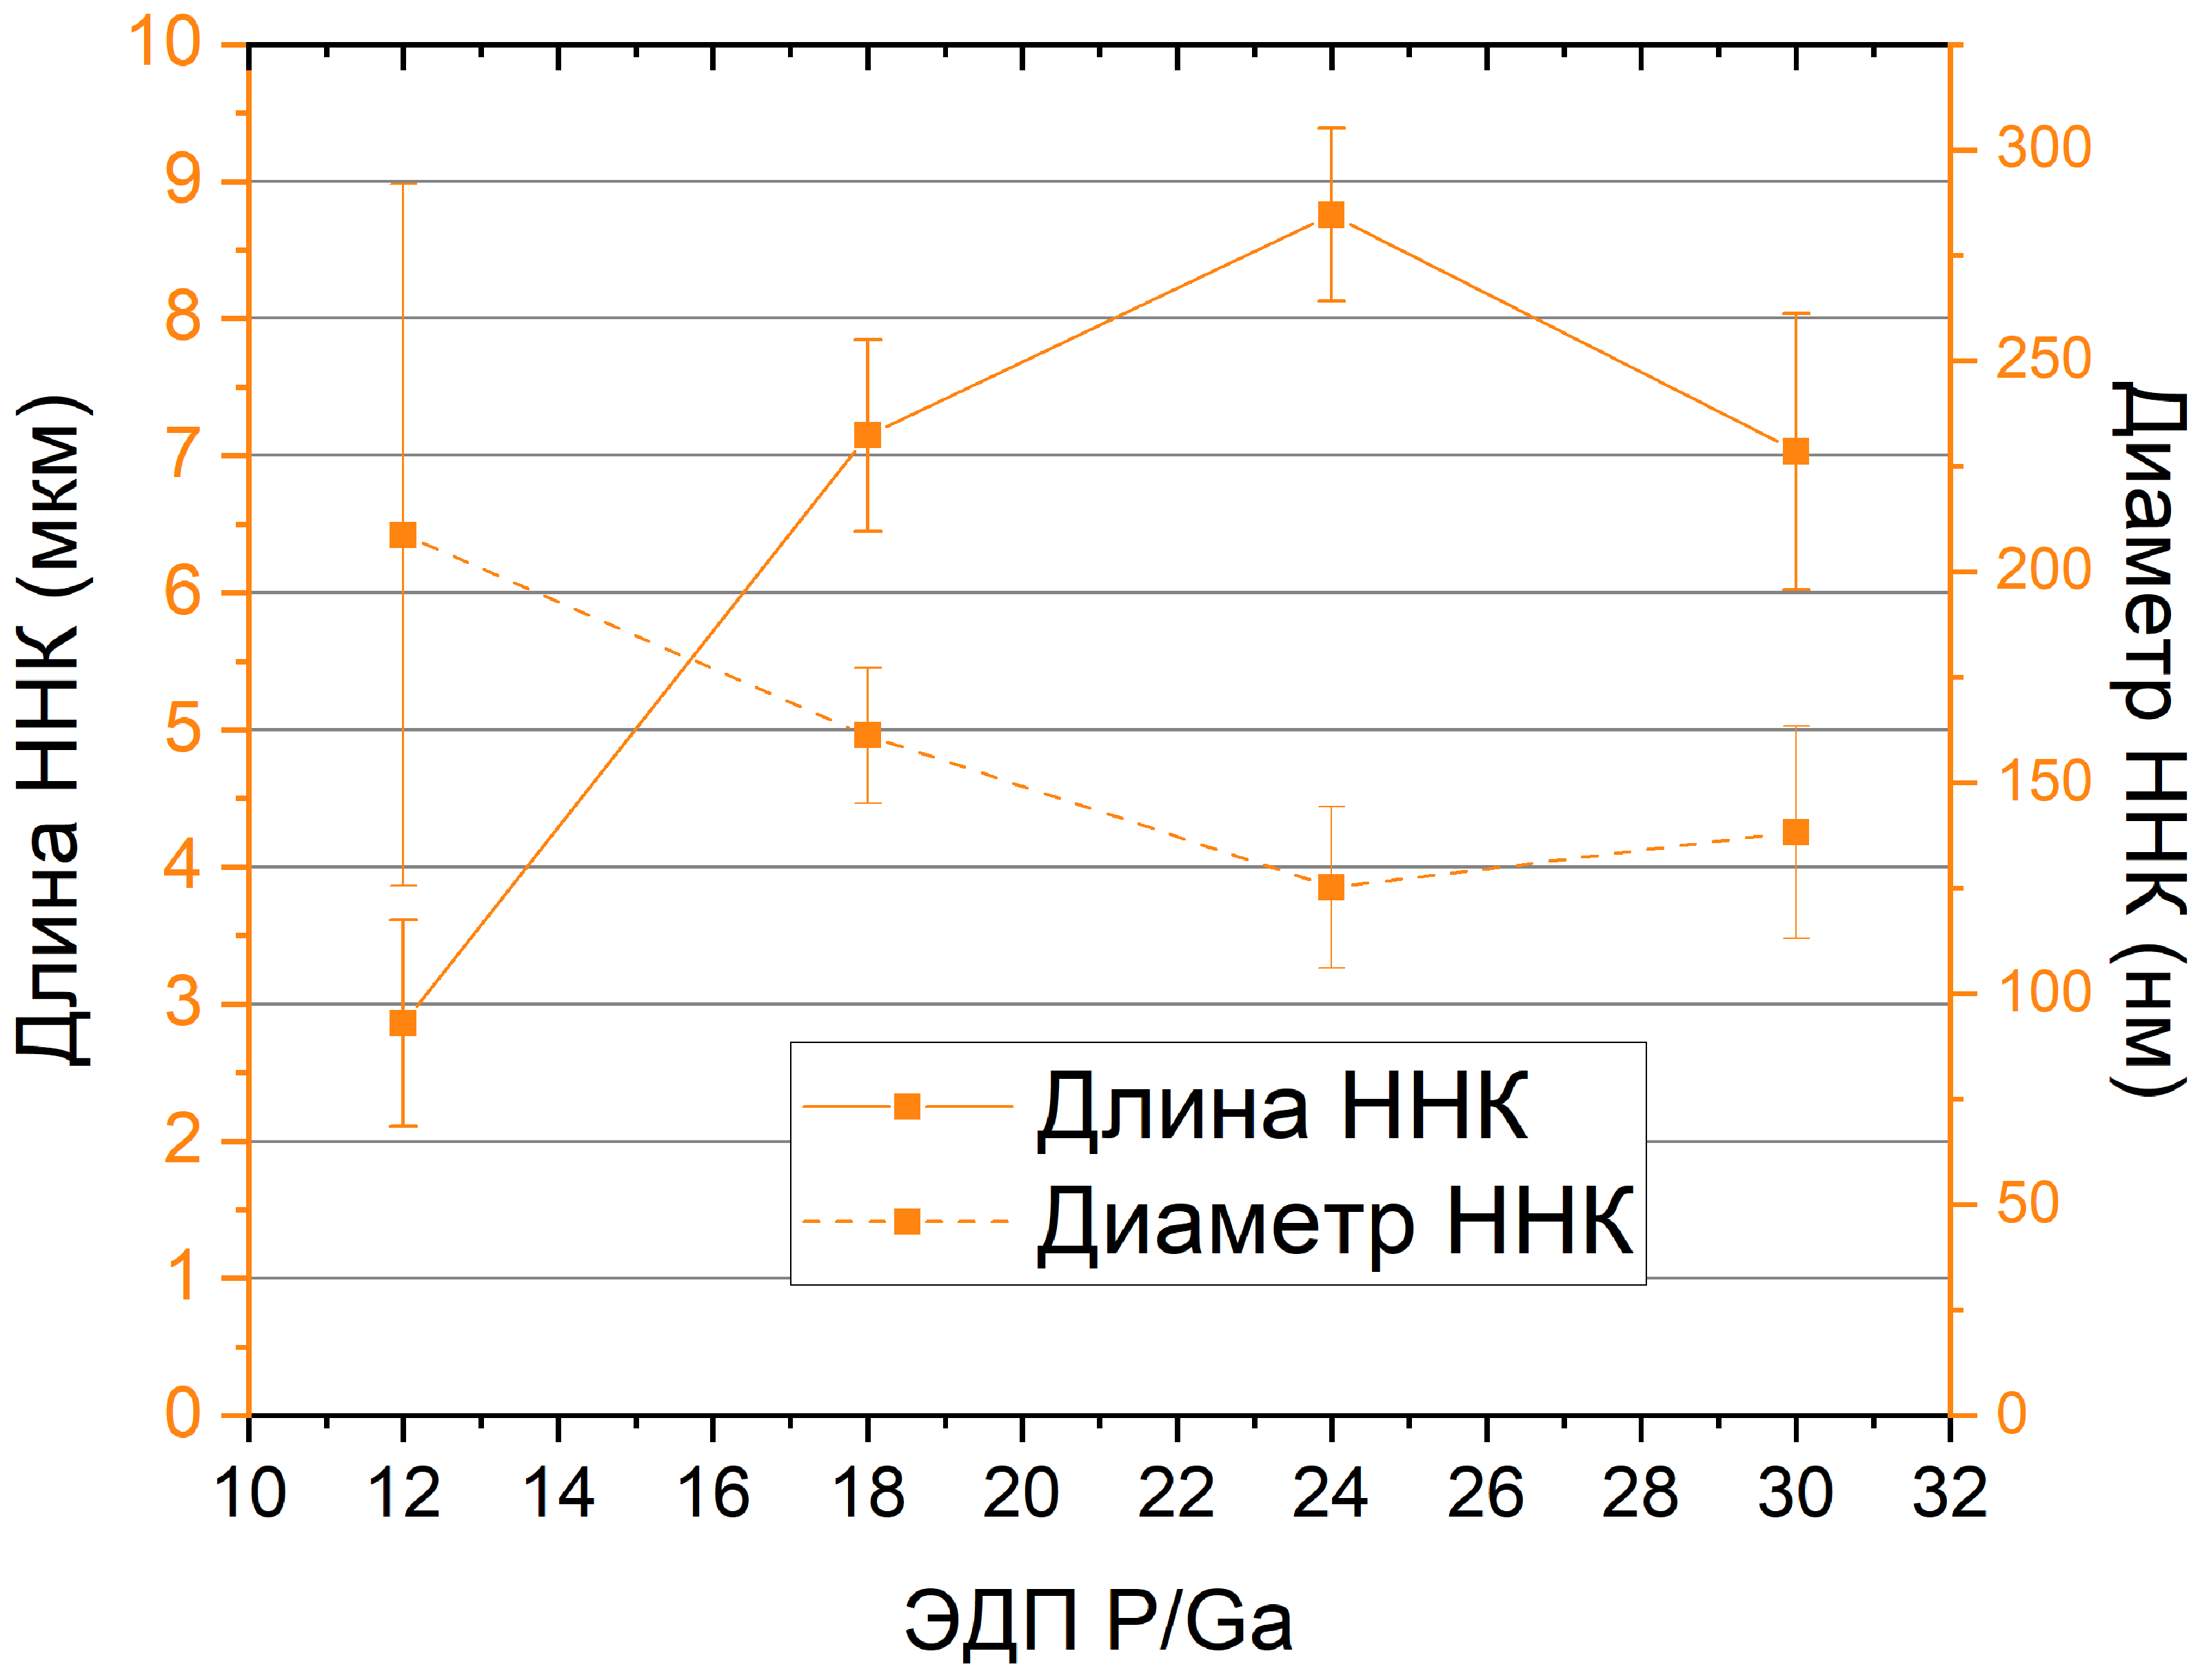
\includegraphics[width=0.48\linewidth]{Image_41_1} } \caption{Зависимость длин и
		диаметров ННК GaP от отношения ЭДП P/Ga (ЭДП Ga поддерживается
постоянным)}\label{fig:Image_41_1} \end{figure}

Поверхностная плотность ННК немонотонно зависит от отношения потоков P/Ga
(см.~рис.~\cref{fig:Image_41_23}), а значит существует оптимальное соотношение
ЭДП P/Ga, позволяющее получить максимальную плотность вертикальных ННК. В
данном исследовании оно составило \(\approx 24\). Можно предположить, что это
связано с размером Ga капель при зарождении ННК: при низком отношении потоков
P/Ga образуются крупные капли, которые имеют больший диффузионный радиус сбора
адатомов с поверхности, что ограничивает образование на этой площади других
капель и ННК. Таким образом, плотность зарождения увеличивается с повышением
отношения потоков P/Ga из-за увеличения плотности капель на поверхности, а при
достижении значений соотношения P/Ga, при котором формируются капли размером
ниже критического~--- зарождение ННК подавляется.

\begin{figure}[ht] \centerfloat{ \subcaptionbox{\label{fig:Image_41_2}}{%
		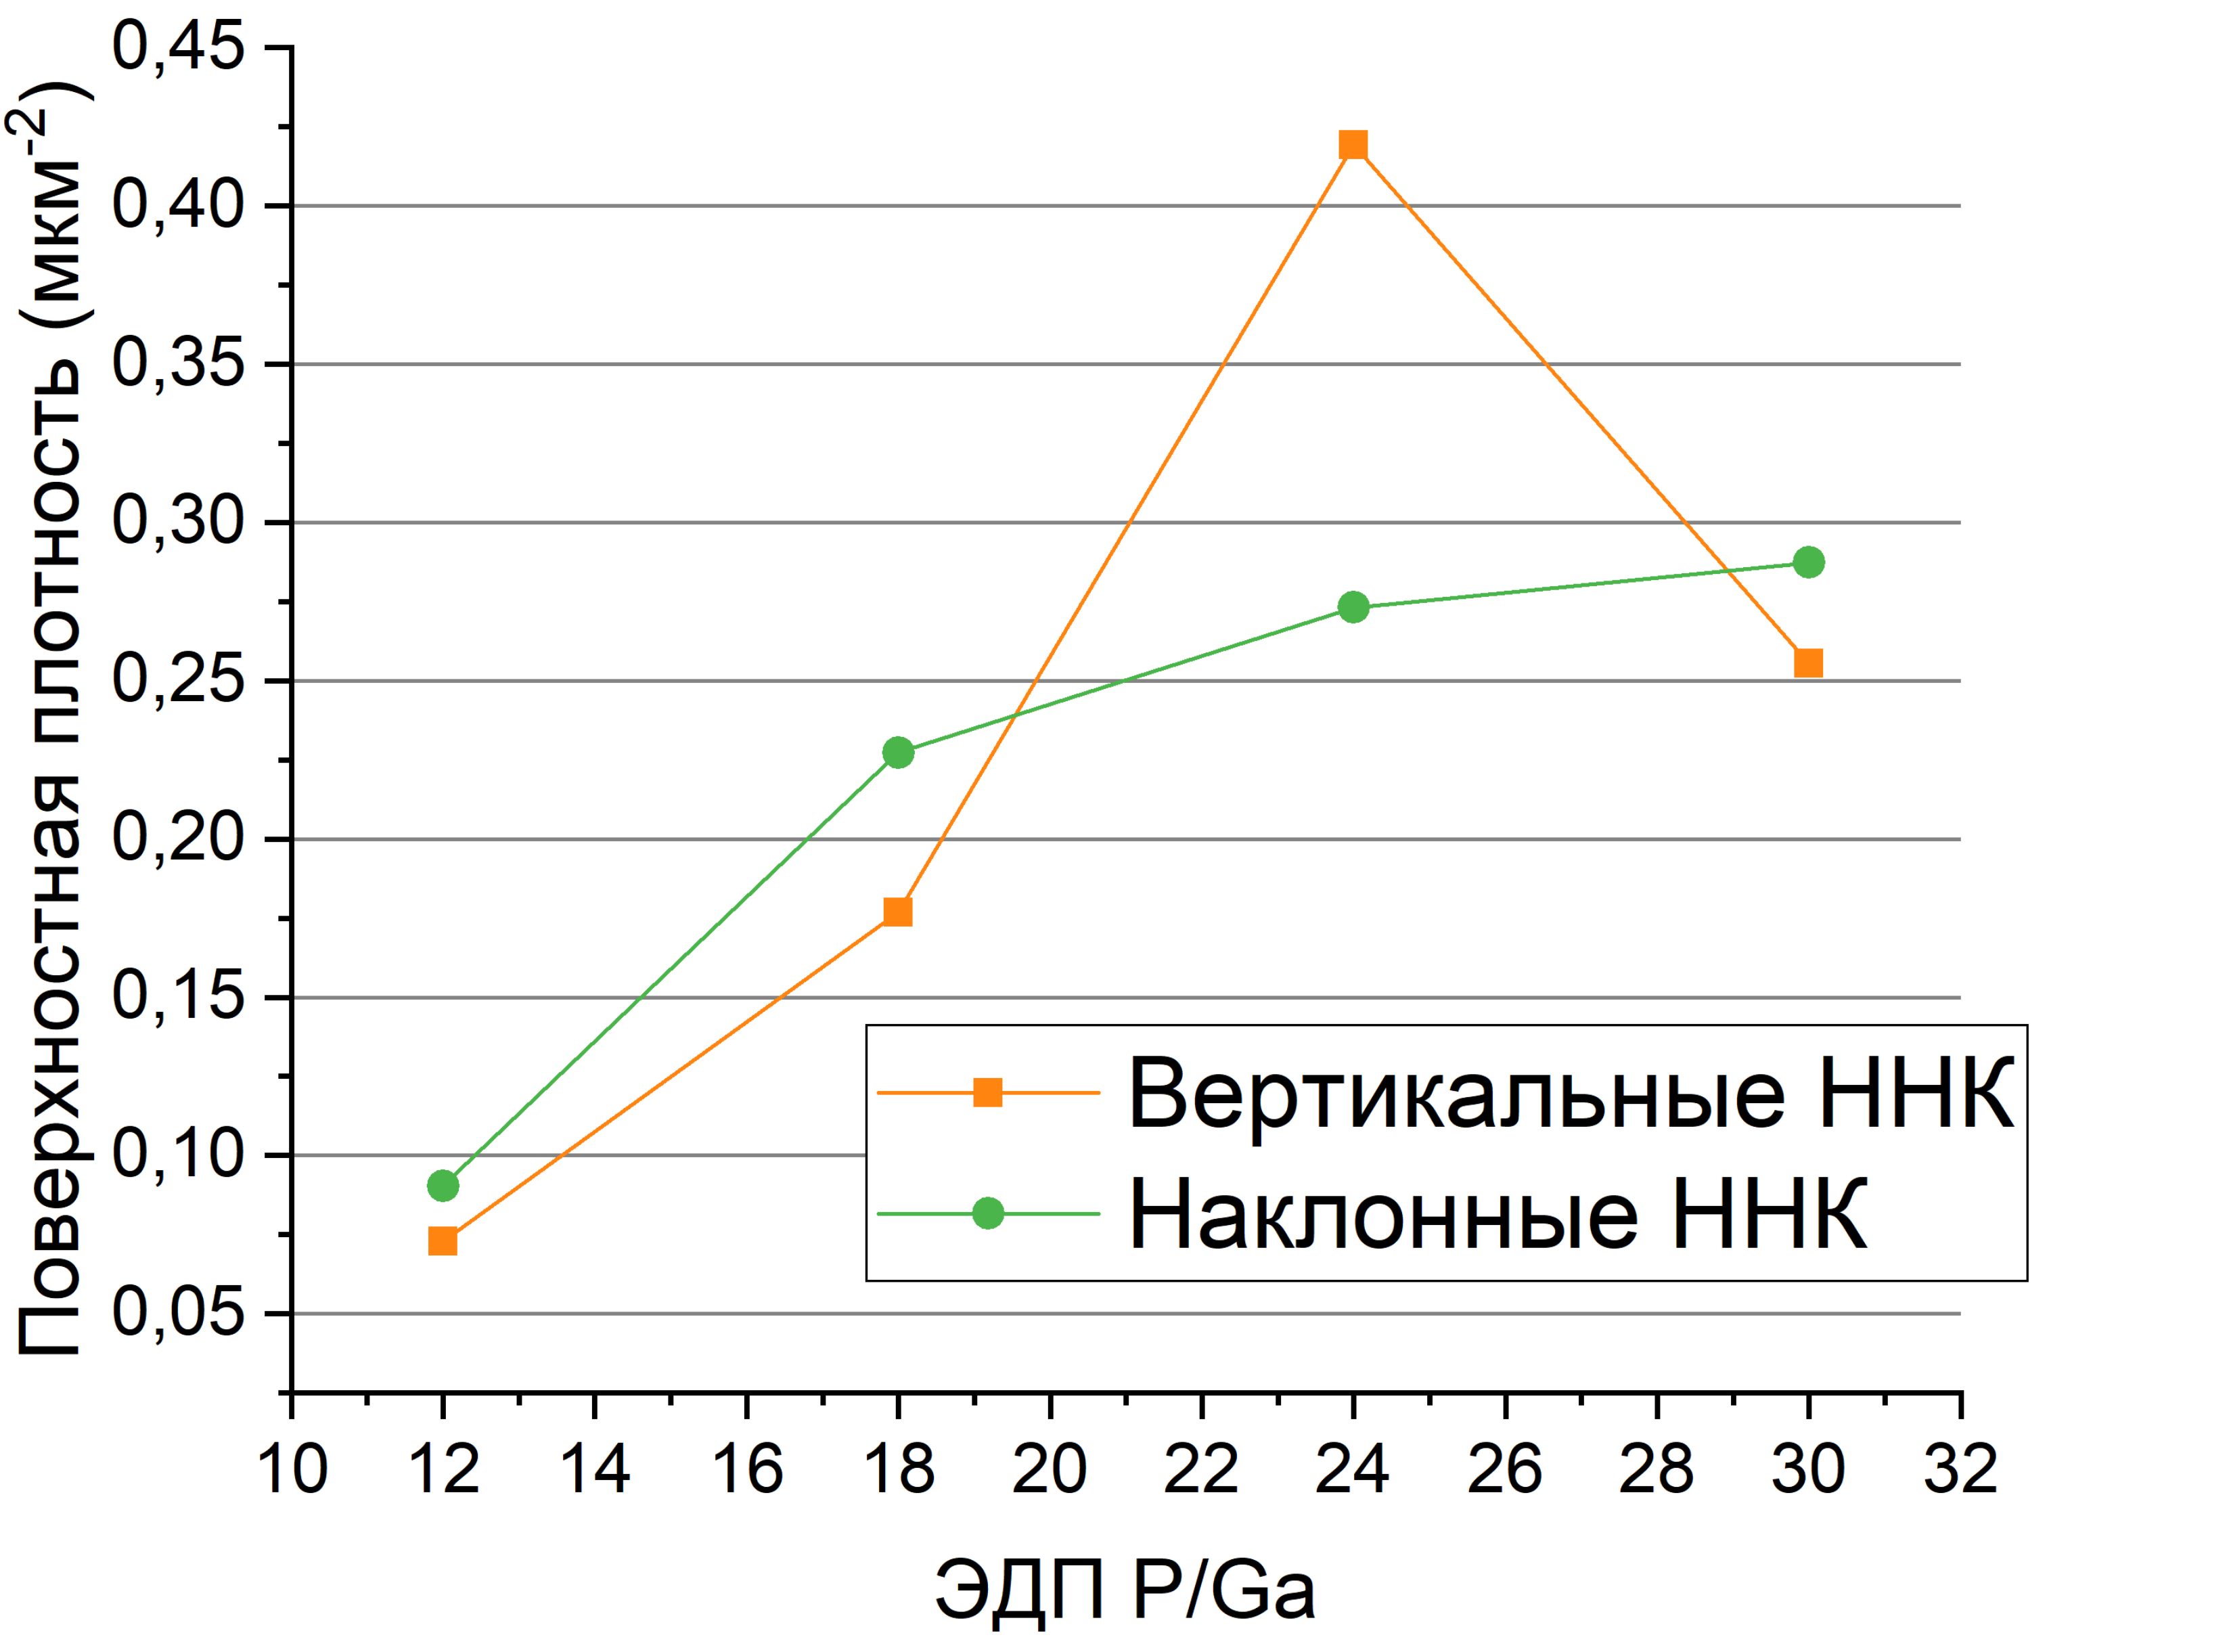
\includegraphics[width=0.48\linewidth]{Image_41_2}}
		\subcaptionbox{\label{fig:Image_41_3}}{%
	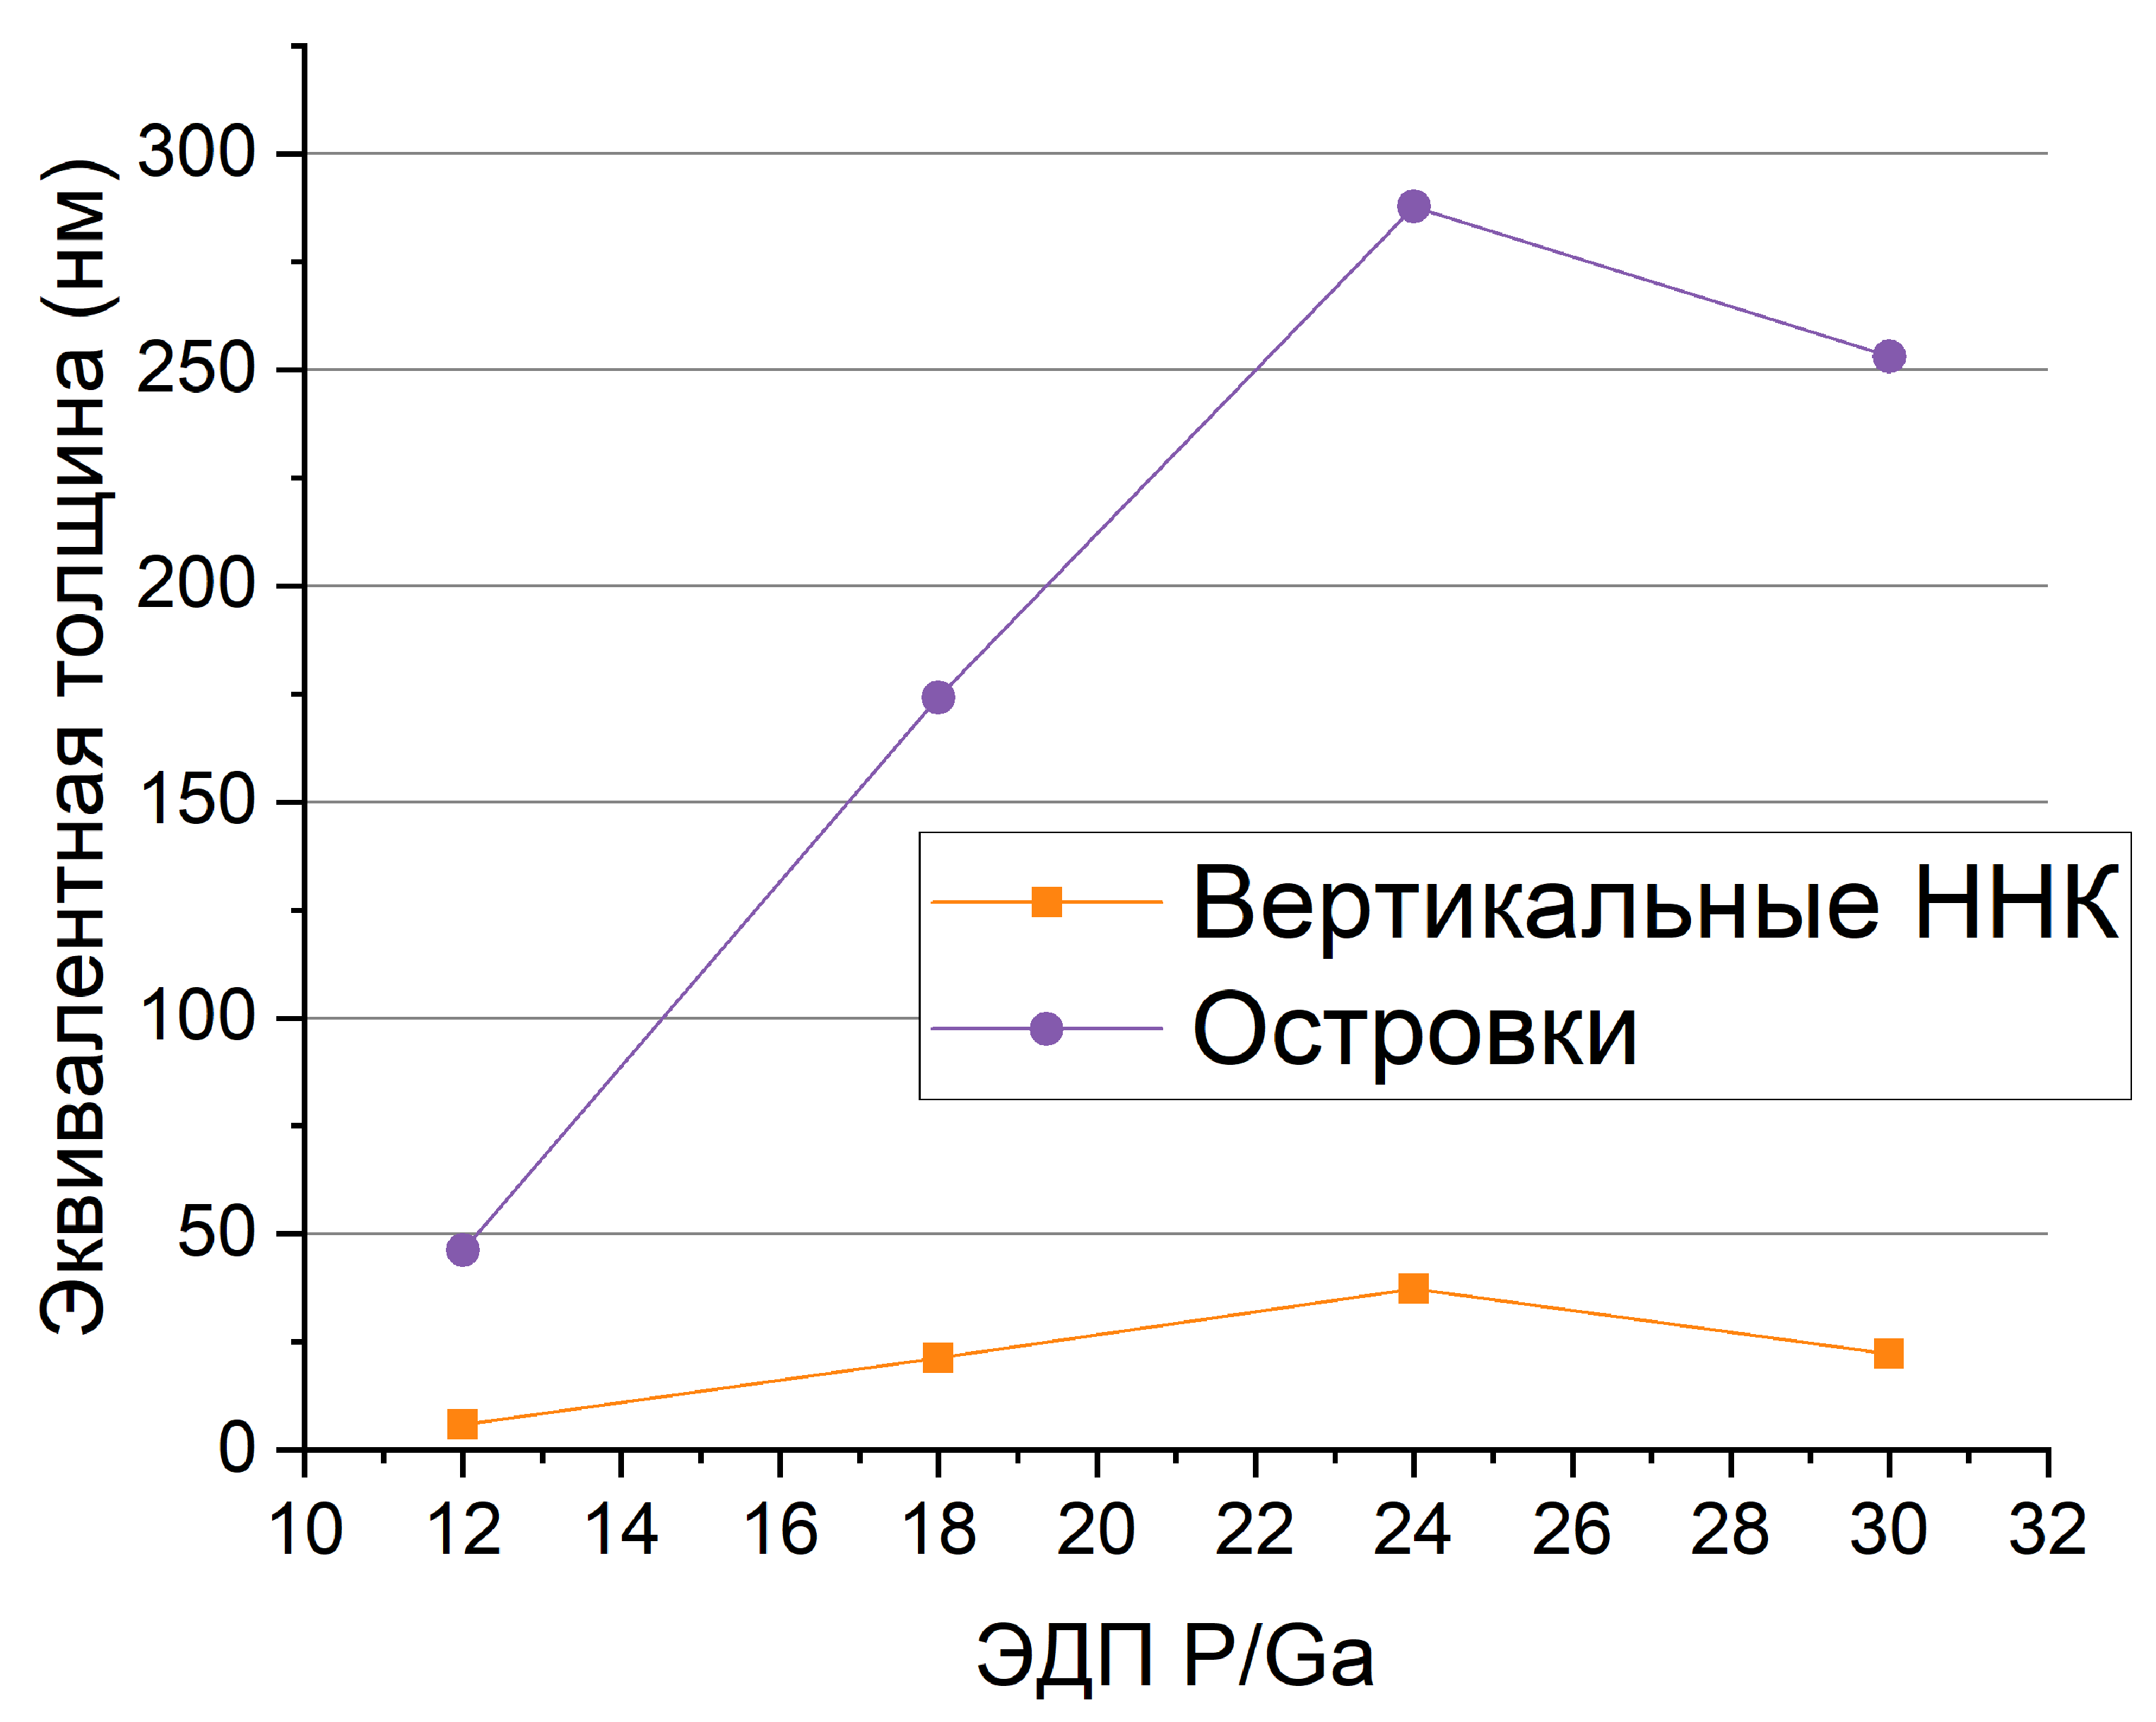
\includegraphics[width=0.48\linewidth]{Image_41_3}} }
	\caption{Зависимость поверхностной плотности~(б) и эквивалентной
		толщины~(в) ННК GaP от отношения ЭДП P/Ga (ЭДП Ga поддерживается
постоянным)}\label{fig:Image_41_23} \end{figure}

\section{Влияние температуры роста и потока Ga}\label{sec:ch5/sec5}

Увеличение температуры роста с 610 до 630~\si{\degreeCelsius} (образец I и II
соответственно) (ЭДП P/Ga ~24, поток Ga 2~отн.~ед.) приводит к резкому
увеличению поверхностной плотности вертикальных ННК и уменьшению плотности
наклонных ННК, при этом плотность островков остаётся практически неизменной
(см.~рис.~\cref{fig:Image_42_1}). Из этого следует, что повышение температуры
способствует образованию зародышей с ориентацией GaP(111)B
(см.~подраздел~\cref{subsec:ch1/sec2/sub4}).

\begin{figure}[ht] \centerfloat{
		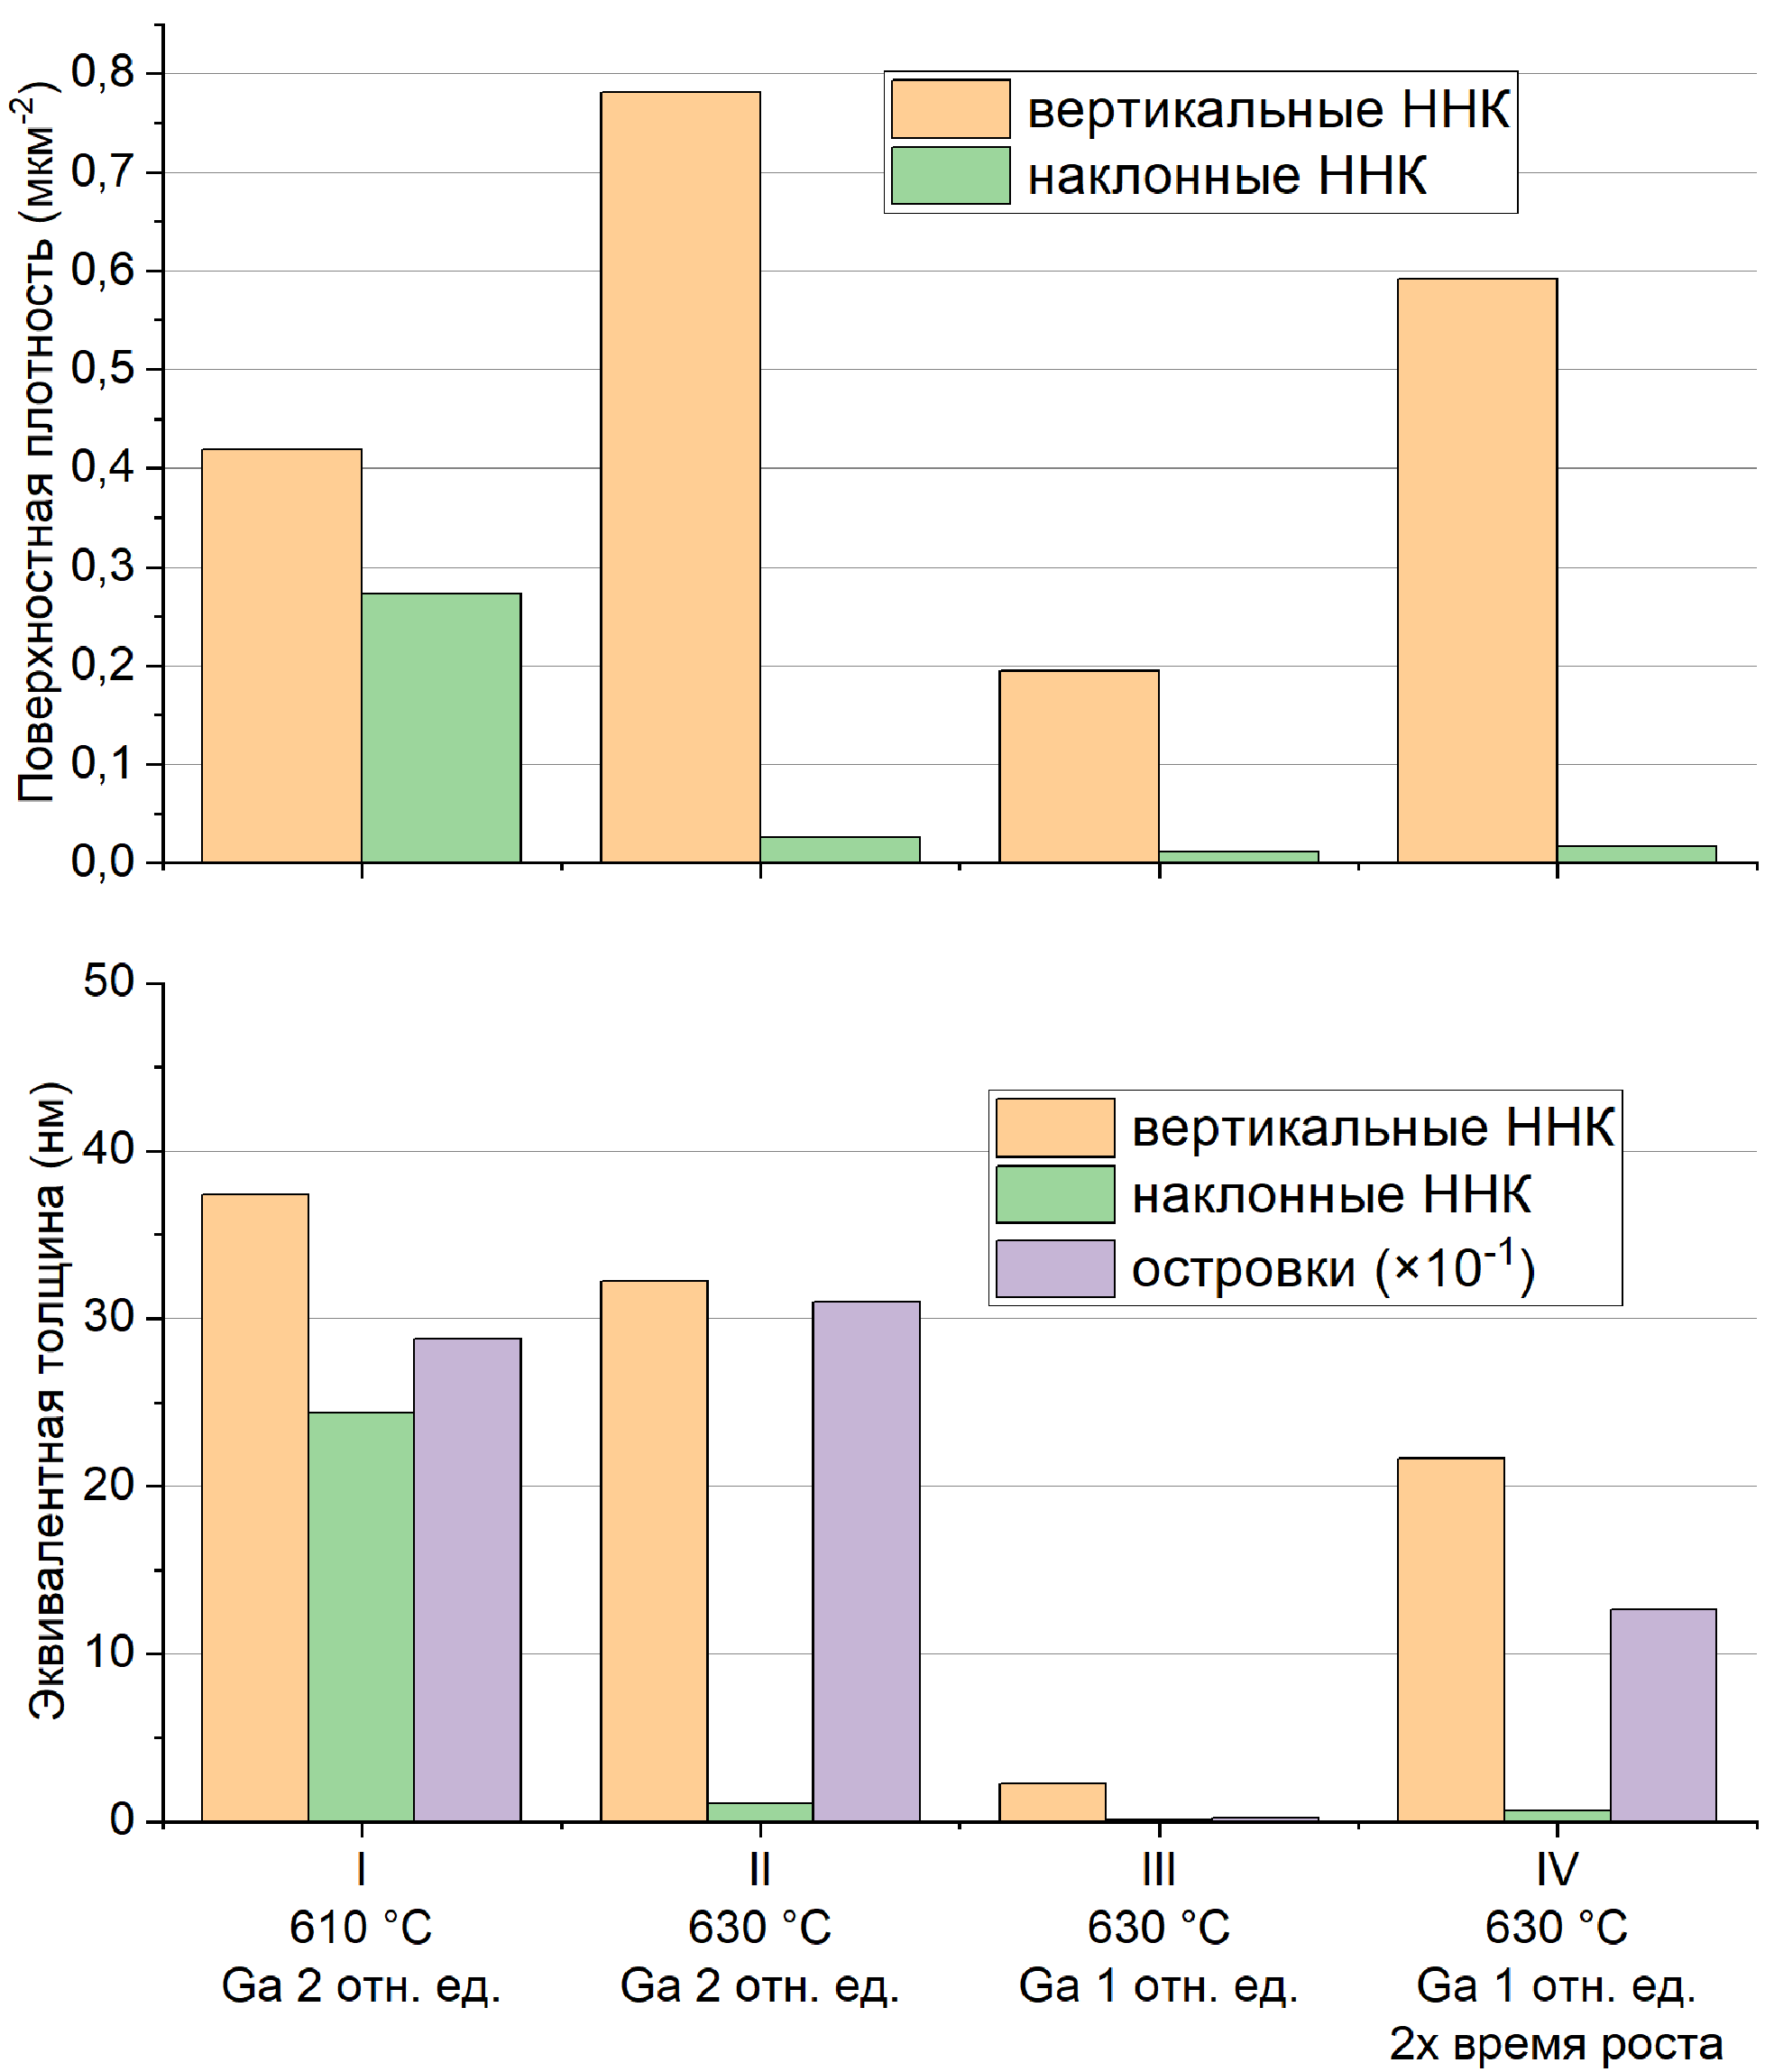
\includegraphics[width=0.6\linewidth]{Image_42_1} } \legend{Образец I:
		массив ННК GaP выращен при температуре роста 610~\si{\degreeCelsius};
		образец II: массив выращен при температуре роста 630~\si{\degreeCelsius};
		образец III: массив выращен при температуре роста 630~\si{\degreeCelsius} и
		потоком Ga 1~отн.~ед., с сохранением соотношения ЭДП P/Ga; образец IV:
		массив выращен при идентичных параметрах с предыдущим, но удвоенным
		временем роста} \caption{Диаграммы поверхностной плотности и эквивалентной
		толщины массивов ННК GaP, выращенных при различных параметрах
синтеза}\label{fig:Image_42_1} \end{figure}

Также, повышение температуры приводит к существенному понижению диаметров ННК
(см.~рис.~\cref{fig:Image_42_2}). Данный эффект может быть объяснён увеличением
десорбции Ga, из-за чего уменьшается стабильный диаметр капли катализатора.

\begin{figure}[ht] \centerfloat{
		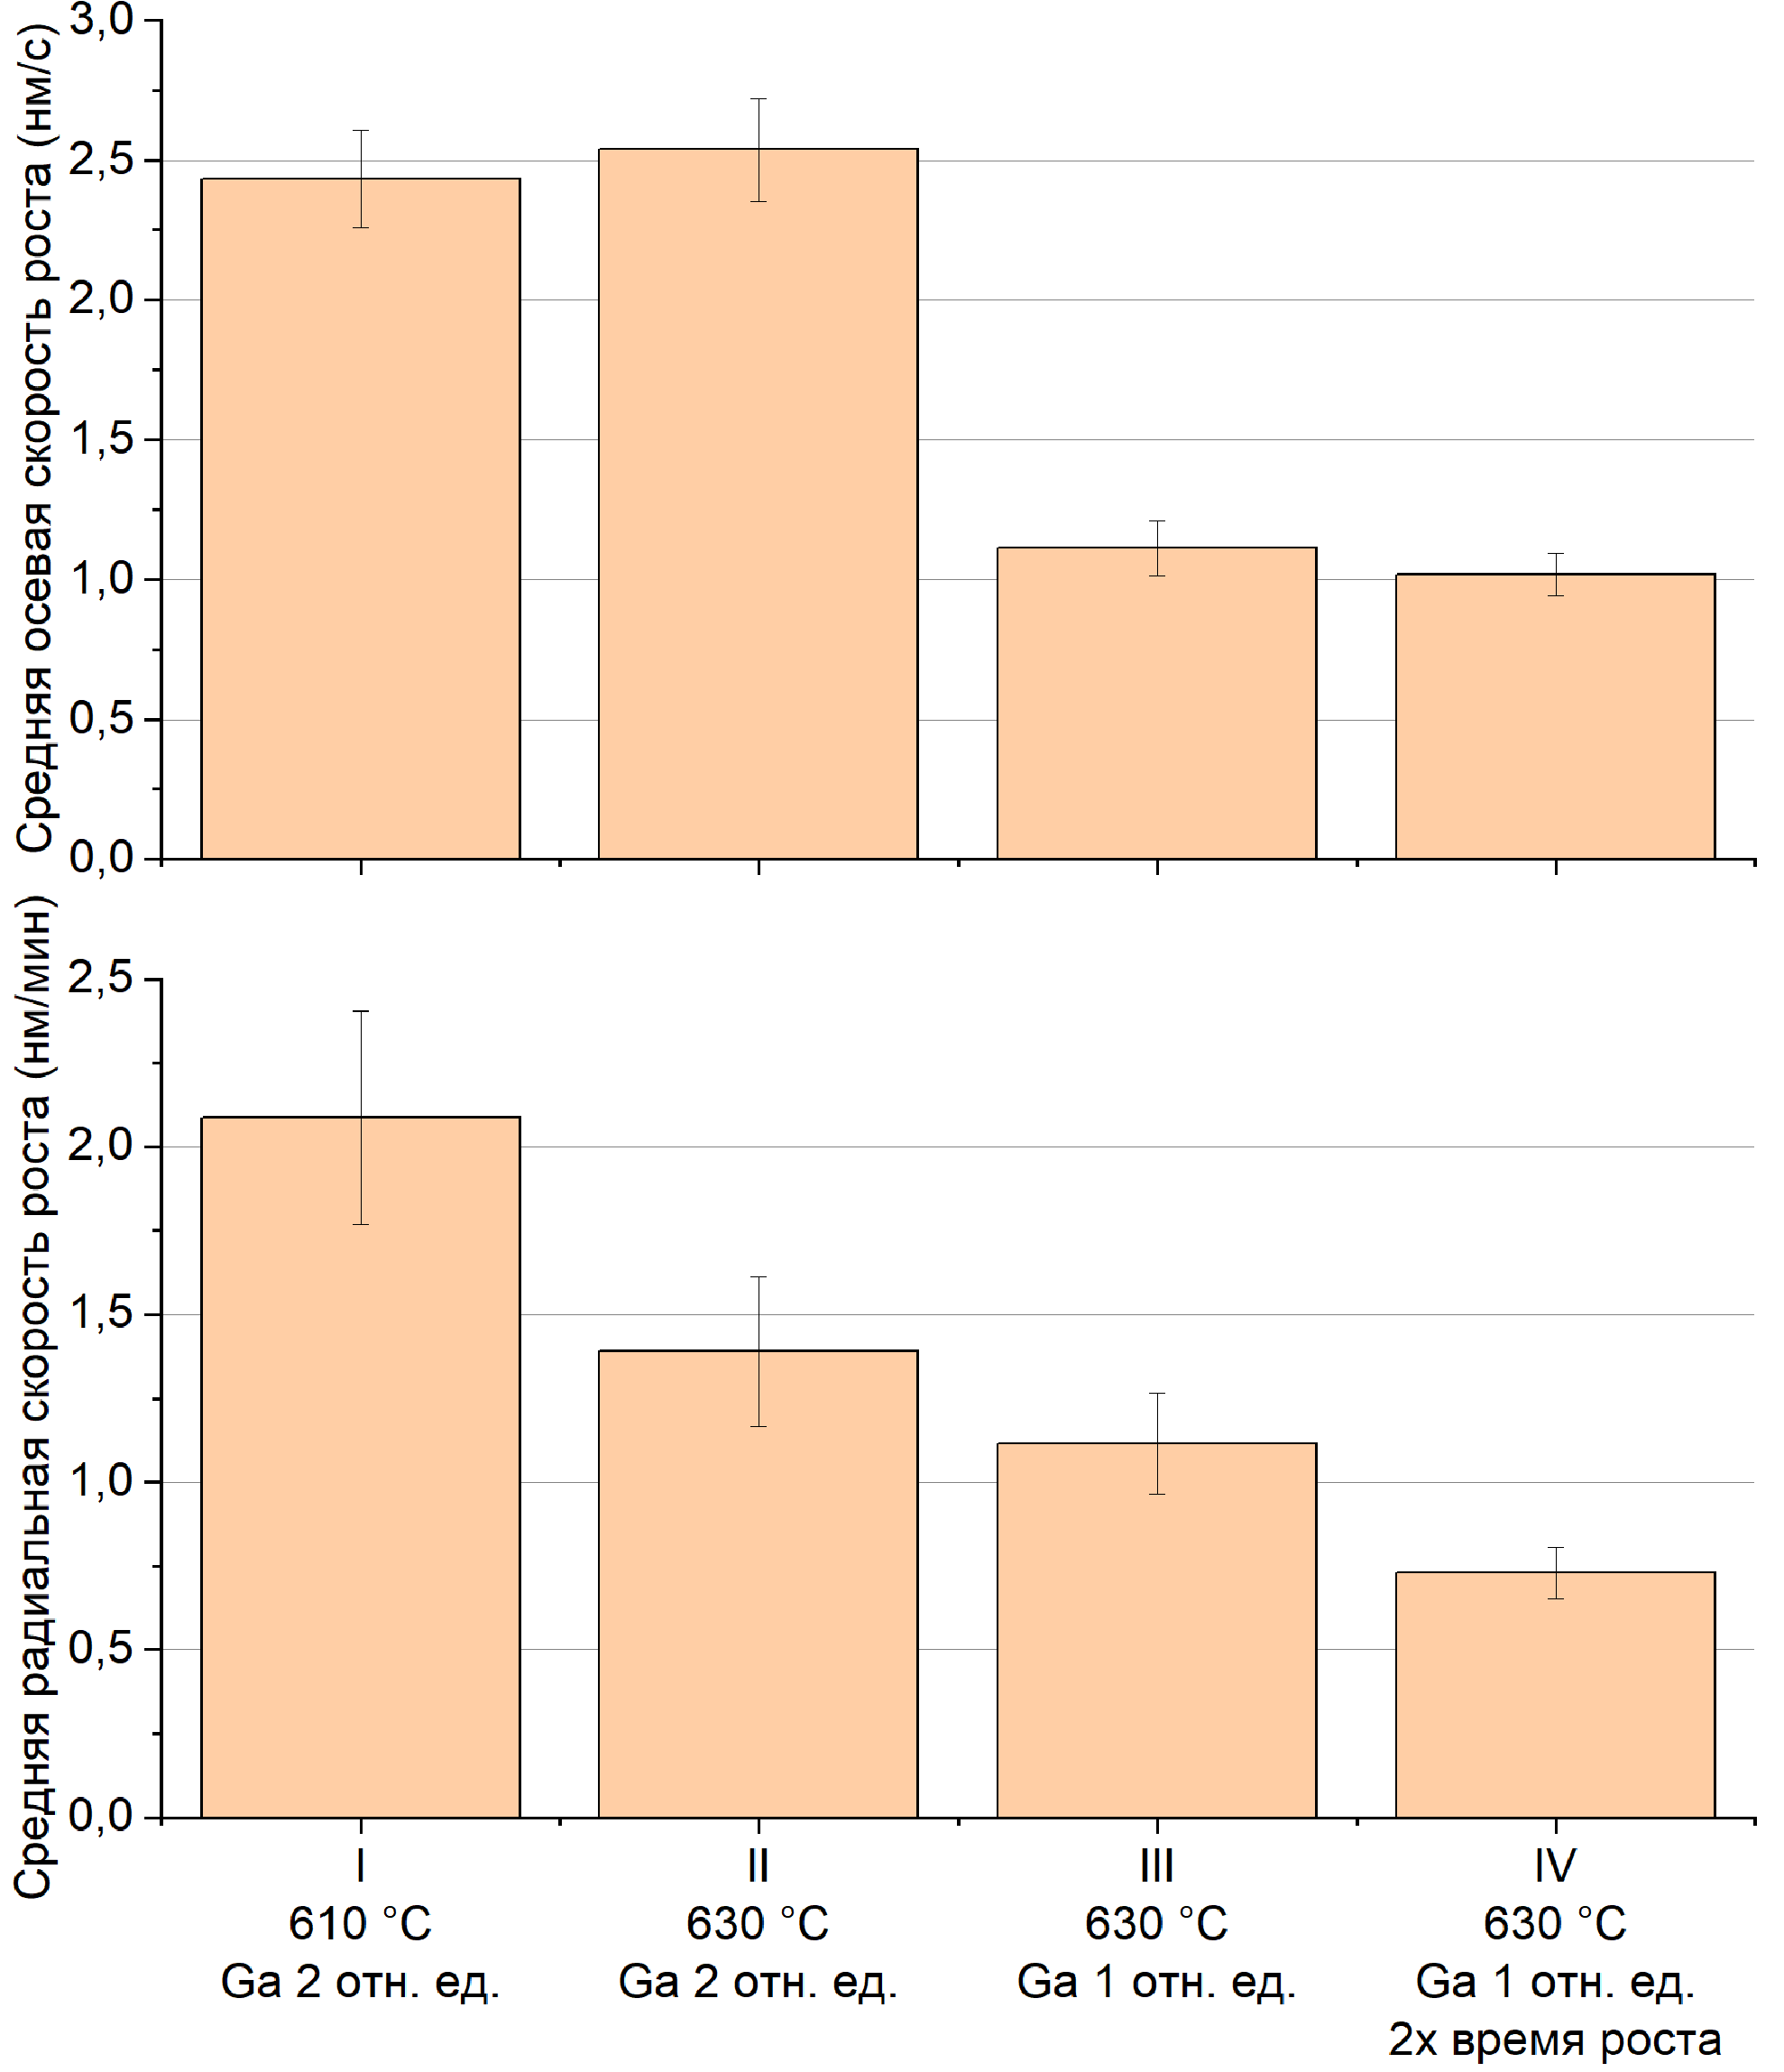
\includegraphics[width=0.6\linewidth]{Image_42_2} } \legend{Образец I:
		массив выращен при температуре роста 610\si{\degreeCelsius};	образец II:
		массив выращен при температуре роста 630\si{\degreeCelsius}; образец III:
		массив выращен при температуре роста 630\si{\degreeCelsius} и потоком Ga
		1~отн.~ед., с сохранением соотношения ЭДП P/Ga; образец IV: массив выращен
	при идентичных параметрах с предыдущим, но удвоенным временем роста}
	\caption{Диаграммы средних по времени скоростей роста ННК GaP образцов,
выращенных при различных параметрах синтеза}\label{fig:Image_42_2} \end{figure}

При уменьшении в два раза абсолютных ЭДП Ga (до~1~отн.~ед.) и P с сохранением
отношения ЭДП P/Ga (образeц III) резко подавляется зарождение паразитных
островков. Из-за резкого снижения количества доступного для роста материала (и,
как следствие, падения длины ННК) был выращен аналогичный образцу III образец
IV, отличающийся удвоенным временем роста для сохранения произведения ЭДП Ga на
время роста как у образца II.

Можно отметить, что эквивалентная толщина GaP у образца IV снижена по сравнению
с образцом II из-за возросшей доли десорбированного P. При этом повысилась доля
материала в форме островков по сравнению с образцом III: эквивалентная толщина
вертикальных ННК за удвоенное время (образец IV) увеличивается в \(\approx
10\)~раз, а островков в \(\approx 60\)~раз.

В сравнении с массивом образца II (поток Ga в 2~раза больше, а время роста в
2~раза ниже) эквивалентная толщина островков массива образца IV снижается в
\(\approx 2,5\)~раза, тогда как эквивалентная толщина вертикальных ННК падает
только в \(\approx 1,5\)~раза. Уменьшение последней вызвано уменьшением длины
(в \(\approx 1,25\)~раза) и плотности ННК (в \(\approx 1,25\)~раза).

\section{Влияние изменения условий формирования в процессе роста}\label{sec:ch5/sec6}

В исследуемом диапазоне условий синтеза диаметр ННК находится в обратной
зависимости от соотношения молекулярных потоков P/Ga
(см.~раздел~\cref{sec:ch5/sec3}) и температуры роста
(см.~раздел~\cref{sec:ch5/sec4}), однако уширение ННК сопровождается
уменьшением плотности и объёмной доли вертикальных ННК. Можно предположить, что
стимулирование роста боковых граней уже сформированного массива плотных
вертикальных ННК возможно путём изменения параметров роста таким образом, чтобы
увеличить размер капли катализатора. Исходя из этого, в разделе рассматривается
рост в две стадии (образец VIII): затравочной стадии (образец V) при высокой
температуре и отношении потоков P/Ga для формирования плотного массива
вертикальных ННК и второй стадии при низком отношении потоков P/Ga за счёт
увеличения потока Ga для увеличения стабильного диаметра капли катализатора.

Параметры роста затравки выбирались исходя из условий формирования плотного
массива вертикальных ННК, низкой плотности паразитных островков и зарождения
большей части массива за время роста первой стадии: время роста~---
2000~\si{\second}, поток Ga в 1~отн.~ед.; соотношение ЭДП P/Ga~--- 30,
температура роста~--- 640~\si{\degreeCelsius}.

Во второй стадии роста  достигалось соотношение ЭДП P/Ga 12 плавным увеличением
ЭДП Ga с 1 до 2,5~отн.~ед. в течение 200~\si{\second} (эквивалентная скорость
роста слоя GaP/Si(001) в избытке P увеличена со 180 до
450~\si{\nano\meter\per\hour}). Время роста второй стадии~---
5000~\si{\second}.

Для оценки влияния второй стадии на морфологию ННК выращены два контрольных
образца со временем роста 7000~\si{\second}: образец VI (без изменения
параметров роста после затравочной стадии) и образец VII (при параметрах роста,
соответствующих второй стадии двухстадийного образца (низкое отношение ЭДП
P/Ga~--- 12 и высокий ЭДП Ga в 2,5~отн.~ед.)).

Поверхностная плотность (см.~рис.~\cref{fig:Image_44_1}) массива ННК на
контрольном образце VI (время роста 7000~\si{\second}) уменьшается по
сравнению с массивом затравок на образце V (время роста 2000~\si{\second},
ростовые параметры идентичны), что указывает на подавление зародышеобразования
после стадии роста затравки. Уменьшение поверхностной плотности массива ННК
может быть вызвано поглощением капли катализатора у некоторых ННК, что
замедляет скорость их роста и уменьшает наблюдаемую плотность массива.

\begin{figure}[ht] \centerfloat{
		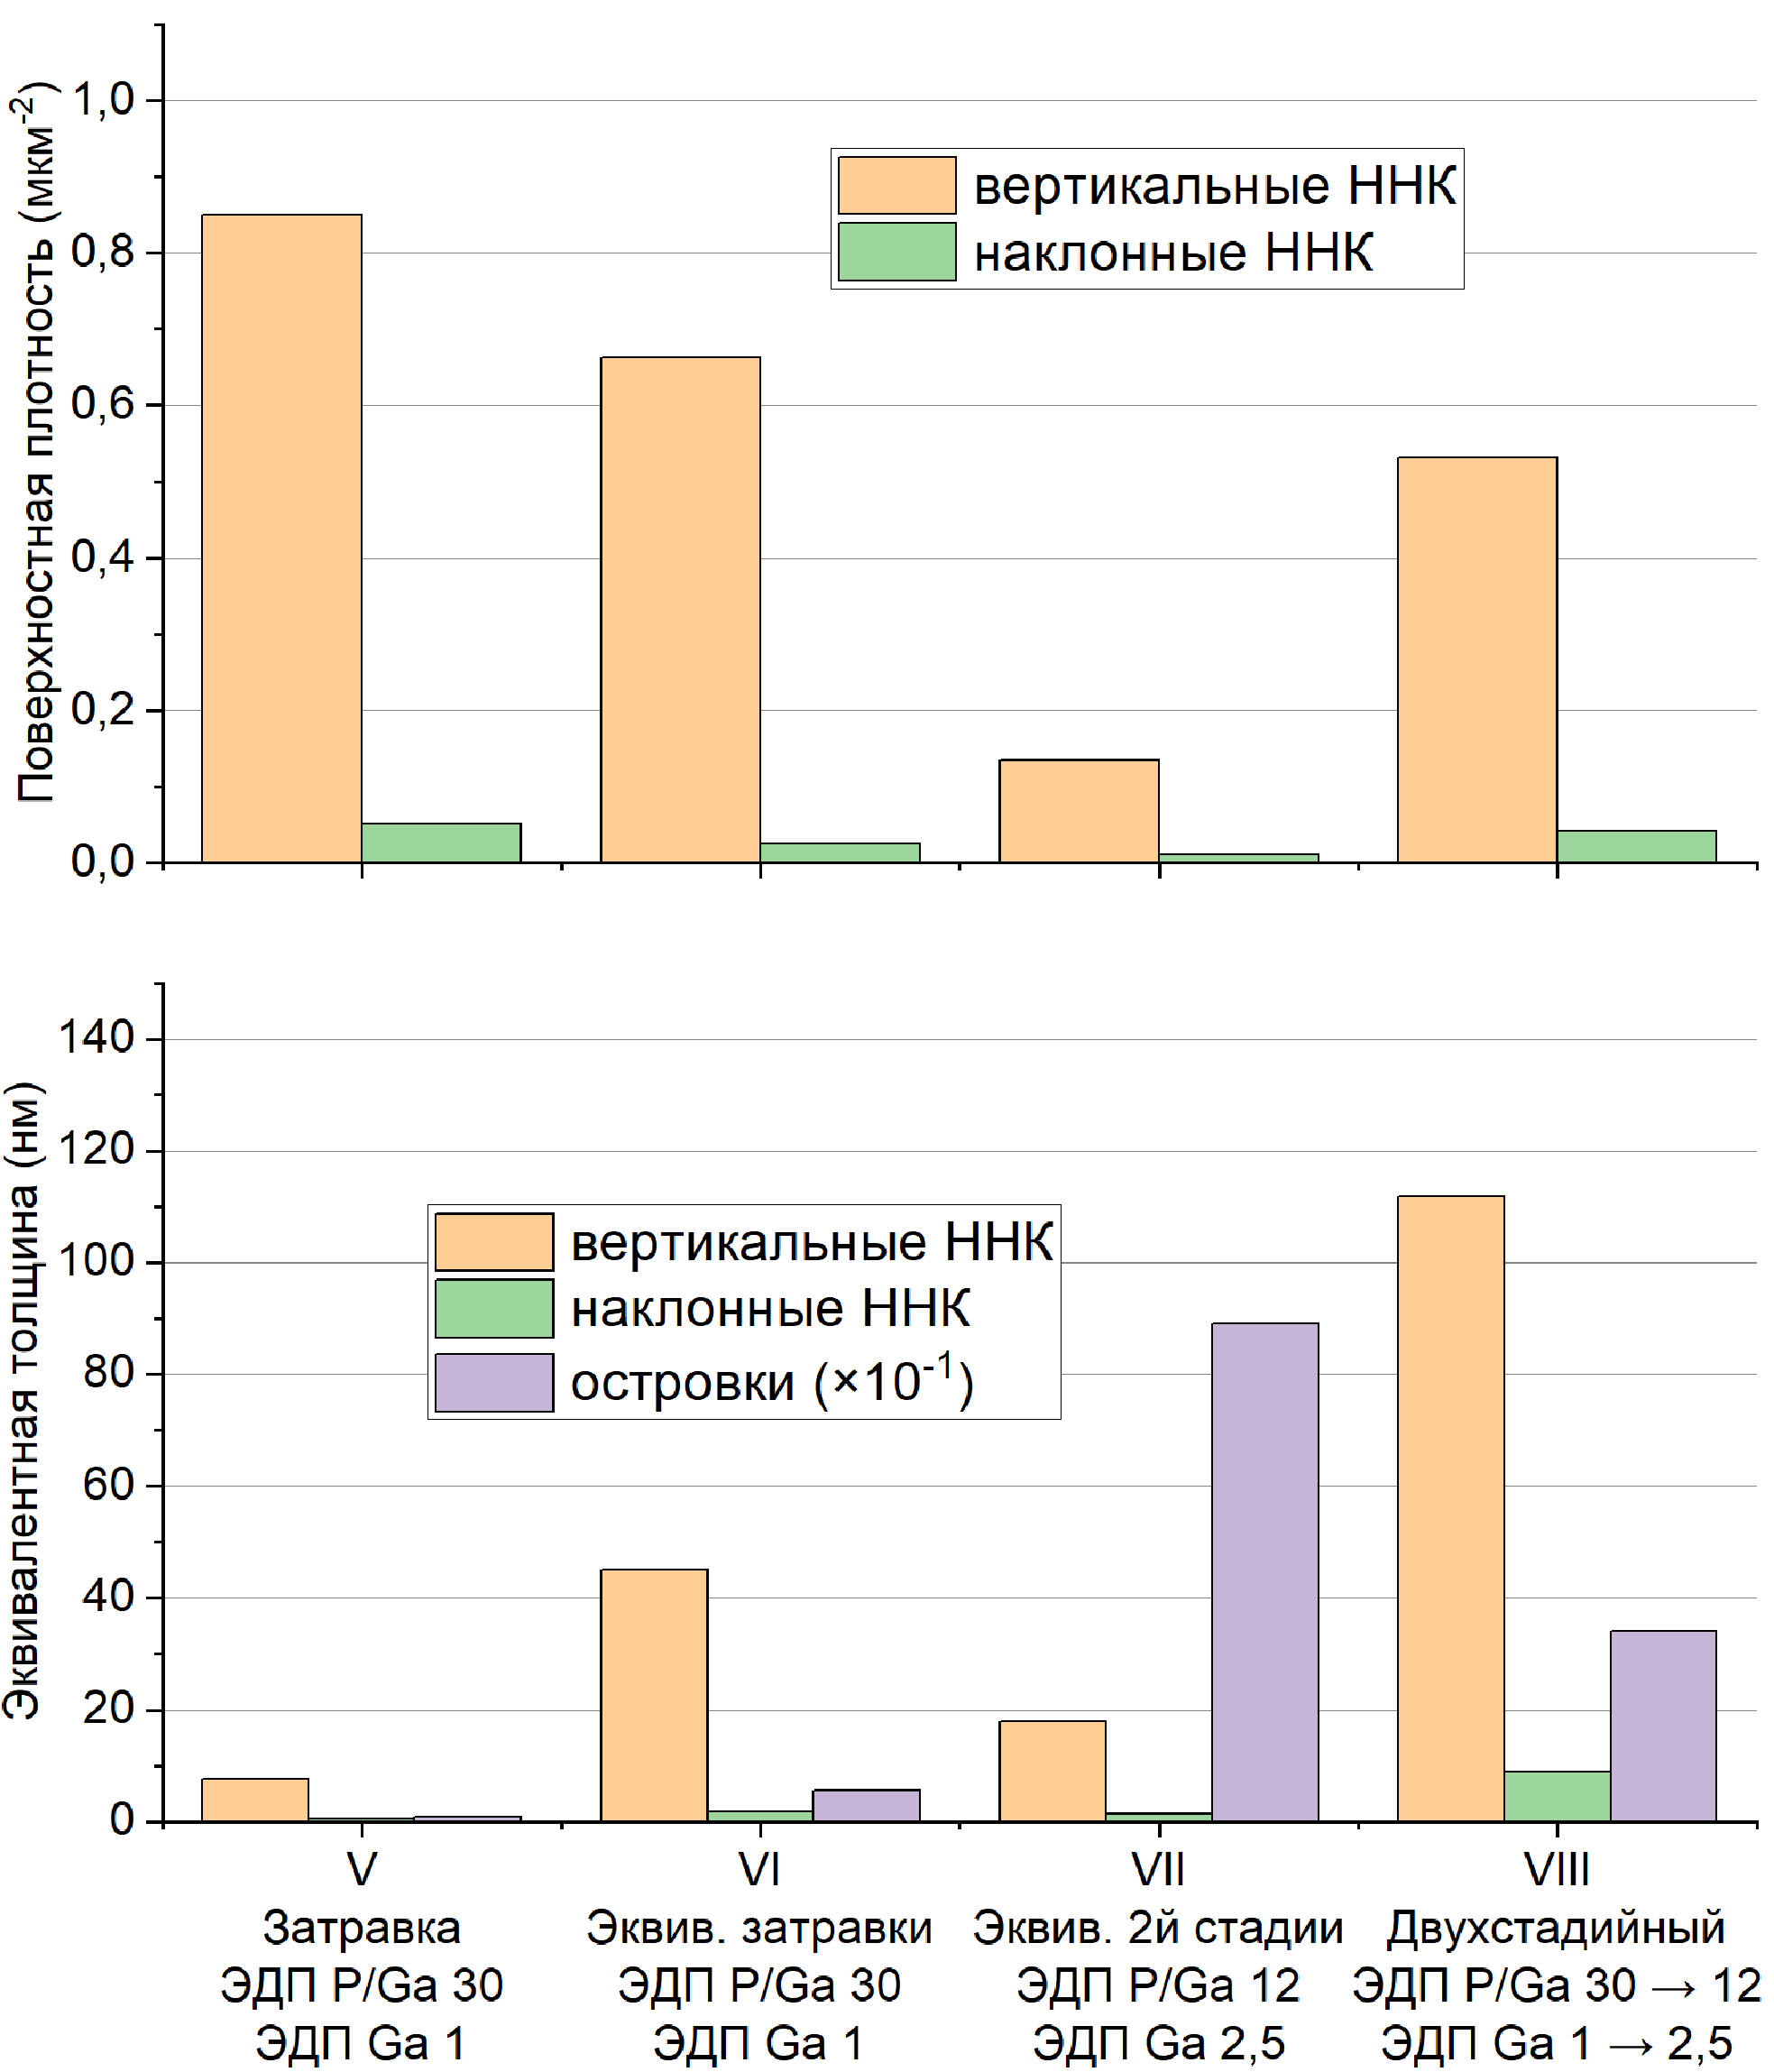
\includegraphics[width=0.6\linewidth]{Image_44_1} } \legend{Образец V:
		затравочный массив (время роста 2000~\si{\second}); образец VI: длинный
		эквивалент затравки без изменения параметров роста (время роста
		7000~\si{\second}); образец VII: выращен при параметрах синтеза,
		эквивалентных второй стадии без затравки (время роста 7000~\si{\second});
		образец VIII: двухстадийный с повышением потока Ga во время второй стадии
		(время роста первой стадии 2000~\si{\second}, время роста второй стадии
		5000~\si{\second})} \caption{Диаграммы поверхностной плотности и
		эквивалентной толщины массивов образцов VI--VIII, показывающие влияние
		изменения размера капли катализатора в процессе роста на поверхностную
плотность и эквивалентную толщина массива)}\label{fig:Image_44_1} \end{figure}

Сравнивая контрольные образцы VI и VII можно отметить, что низкое соотношение
потоков P/Ga ожидаемо снижает плотность ННК (подробнее
см.~раздел~\cref{sec:ch5/sec3})~--- большая часть поглощённого
материала кристаллизуется в виде островков. Сравнивая контрольный образец VII
с двухстадийным образцом VIII, можно отметить роль затравки~--- формирование
плотного массива с низкой плотностью островков.

Можно предположить, что скорость роста ННК контрольного образца VII выше в
сравнении с ННК образца VI из-за недостатка Ga
(см.~раздел~\cref{sec:ch5/sec3}), а скорость роста ННК
двухстадийного образца VIII выше скорости роста ННК контрольного образца VII
из-за подавления образования островков, а значит большем количестве адатомов
Ga, которые могут попасть попасть каплю или встроиться в боковую грань ННК
(см.~рис.~\cref{fig:Image_44_2}).

\begin{figure}[ht] \centerfloat{
		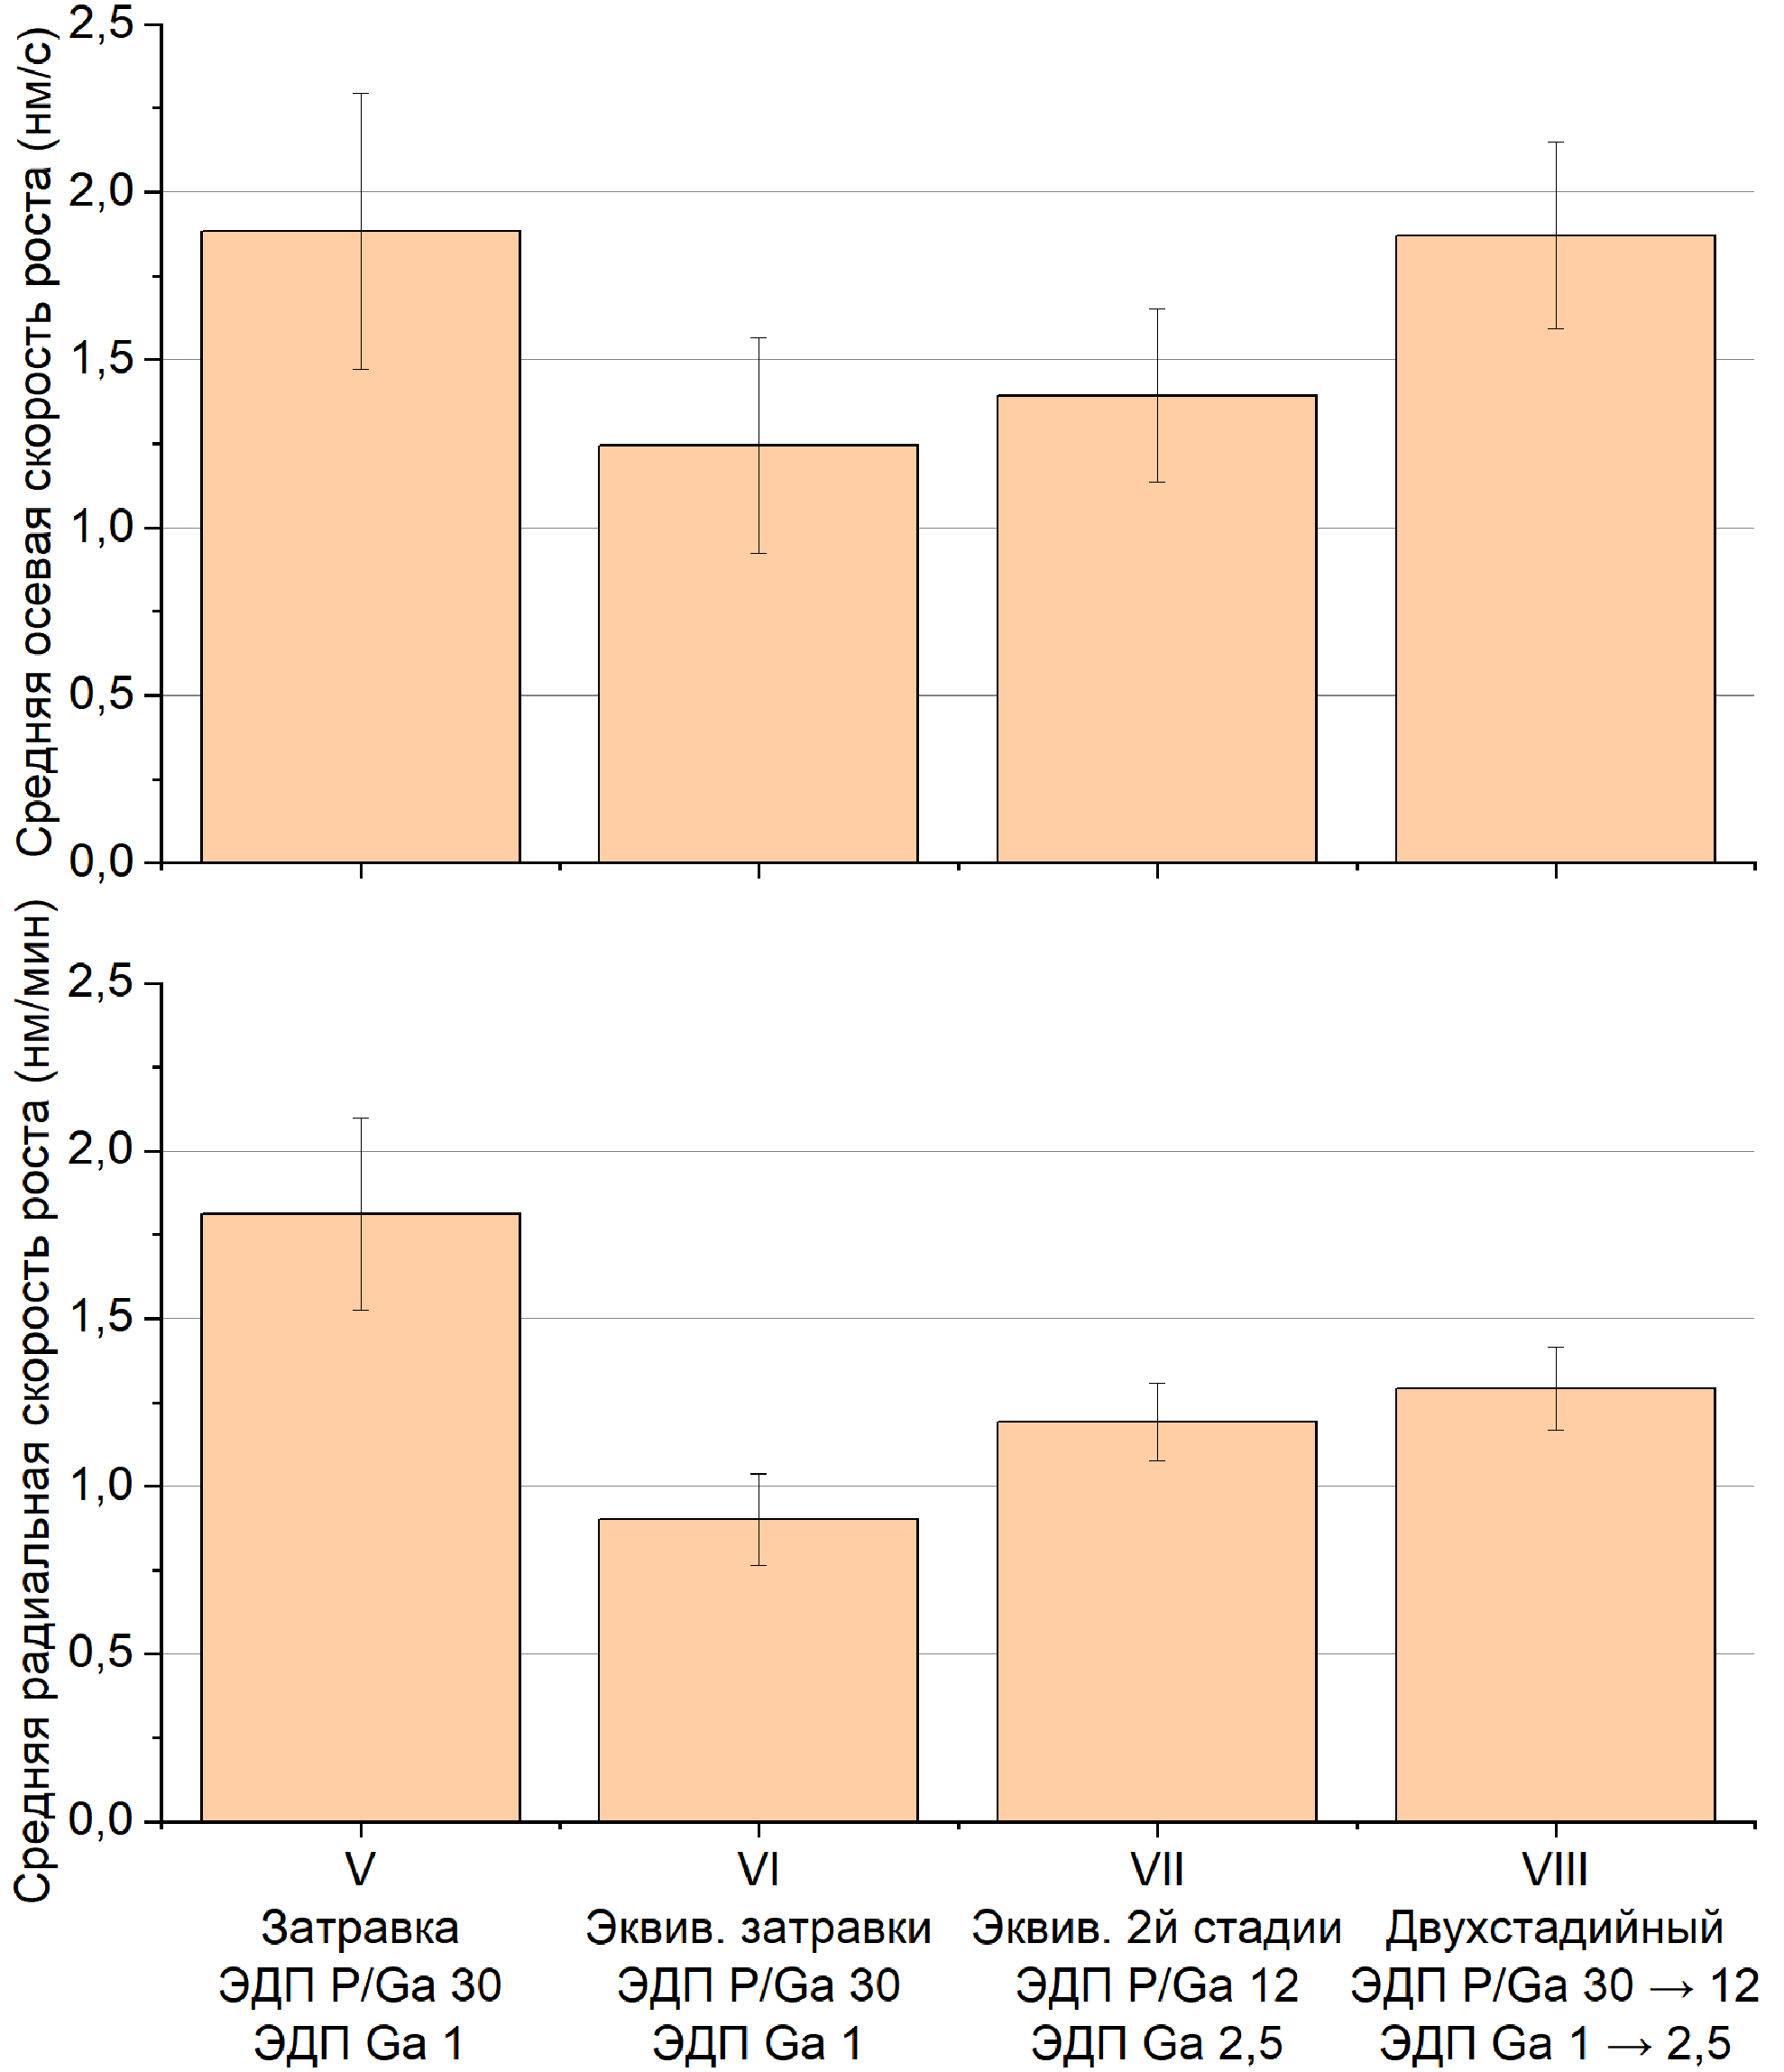
\includegraphics[width=0.6\linewidth]{Image_44_2} } \legend{Образец V:
		затравочный массив (время роста 2000~\si{\second}); образец VI: длинный
		эквивалент затравки без изменения параметров роста (время роста
		7000~\si{\second}); образец VII: выращен при параметрах синтеза,
		эквивалентных второй стадии без затравки (время роста 7000~\si{\second});
		образец VIII: двухстадийный с повышением потока Ga во время второй стадии
		(время роста первой стадии 2000~\si{\second}, время роста второй стадии
		5000~\si{\second})} \caption{Диаграммы средних скоростей роста образцов
		VI--VIII, показывающие влияние изменения размера капли катализатора в
процессе роста на среднюю скорость роста)}\label{fig:Image_44_2} \end{figure}

Аспектное отношение длина/диаметр ННК образцов VI, VII и VIII отличается слабо,
однако если учесть, что оно зависит от длины ННК
(см.~рис.~\cref{fig:Image_43_1}), и тот факт, что ННК двухстадийного образца
VIII выше ННК контрольного образца VII, то можно прийти к выводу, что при
одинаковой длине ННК, двухстадийный метод позволяет синтезировать ННК с большим
диаметром (см.~рис.~\cref{fig:Image_45}).

\begin{figure}[ht] \centerfloat{
		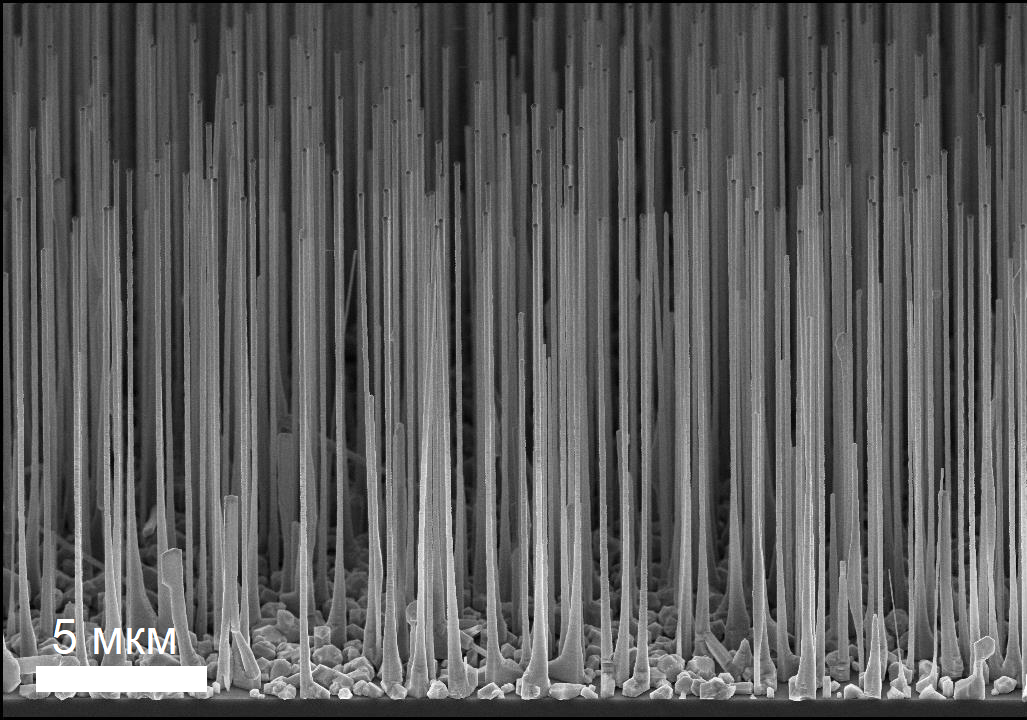
\includegraphics[width=0.6\linewidth]{Image_45} } \caption{РЭМ изображение
	двухстадийного образца VIII (угол наклона 30{\textdegree})}\label{fig:Image_45}
\end{figure}

ННК всех образцов имеют небольшое сужение к вершине (угол конуса
0,2--0,4{\textdegree}), а значит, несмотря на увеличение капель в результате
увеличения потока Ga, наблюдается равномерный радиальный рост по всей длине
ННК. Можно предположить, что увеличение каталитической капли вызывает
увеличение площади верхней грани ННК, тем самым формируя атомные ступени в
самой верхней части ННК. Эти ступени служат энергетически выгодными местами для
встраивания адатомов и приводит к росту в режиме встраивания адатомов в края
ступеней (step-flow) на боковых гранях ННК. При этом происходит движением края
ступени от вершины к основанию ННК и радиальному росту с сохранением однородной
по длине ННК толщиной.

\section{Кристаллическая структура ННК}\label{sec:ch5/sec7}

Исходя из картины ДБЭ ННК растут эпитаксиально со структурой ZB вдоль
[111]\textsubscript{Si} с двойникованием на 180{\textdegree} вокруг направления
роста [111]\textsubscript{GaP} (см.~рис.~\cref{fig:Image_46}). Так как ННК
выращены на подложках с разориентацией 4{\textdegree}, они имеют на
изображениях РЭМ наклон на 2{\textdegree} или 4{\textdegree} к нормали
плоскости подложки в зависимости от ориентации края скола.

\begin{figure}[ht] \centerfloat{
		температура роста 630\si{\degreeCelsius};

		рост 7200~\si{\second} при ЭДП P/Ga 18

		\subcaptionbox{\label{fig:Image_46_1}}{%
		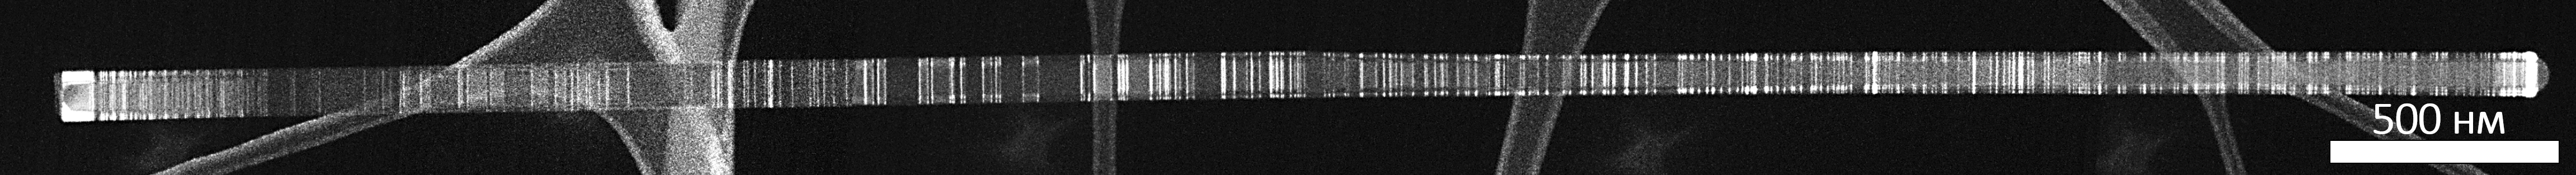
\includegraphics[width=1\linewidth]{Image_46_1}}

		температура роста 640\si{\degreeCelsius};

		рост 5000~\si{\second} при ЭДП P/Ga 24

		\subcaptionbox{\label{fig:Image_46_2}}{%
		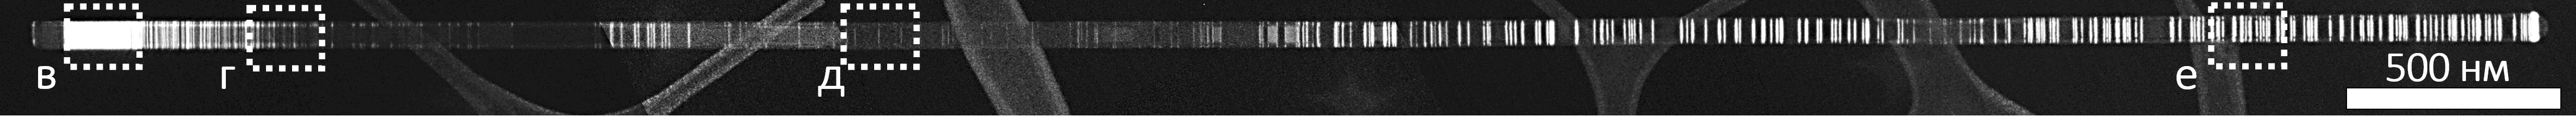
\includegraphics[width=1\linewidth]{Image_46_2}}

		\subcaptionbox{\label{fig:Image_46_3}}{%
		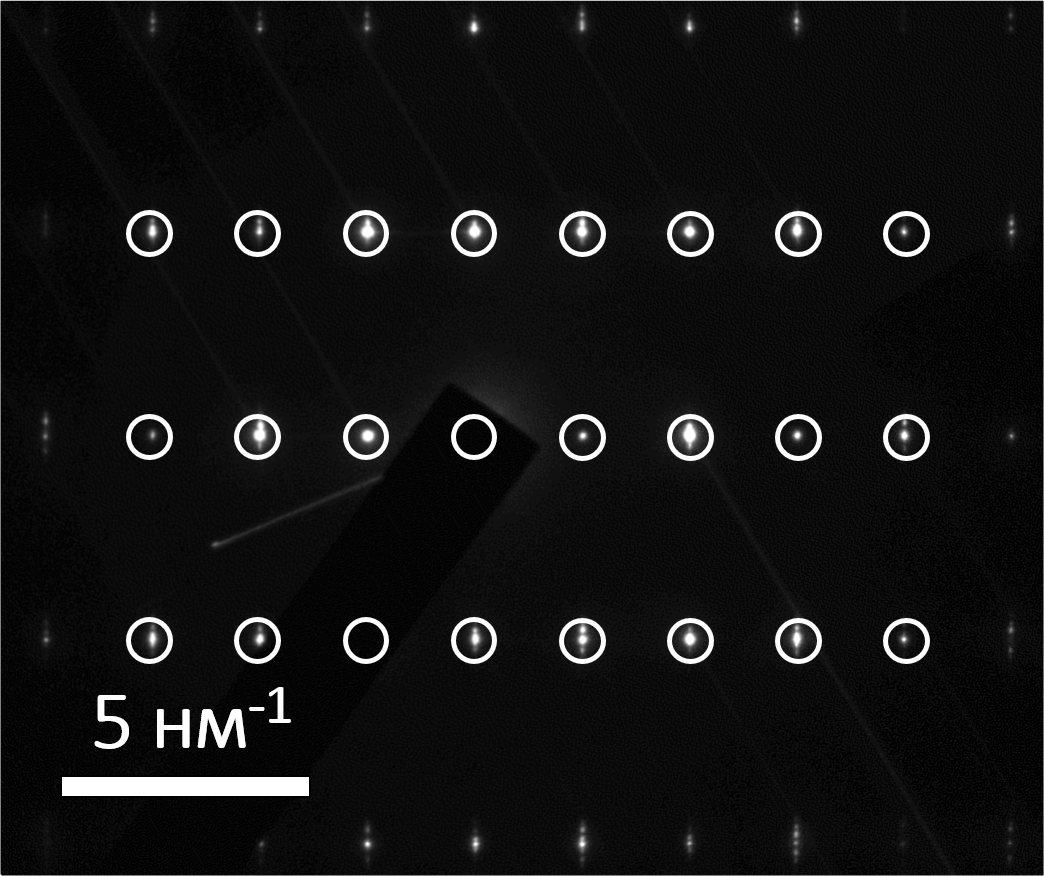
\includegraphics[width=0.24\linewidth]{Image_46_3}}
		\subcaptionbox{\label{fig:Image_46_4}}{%
		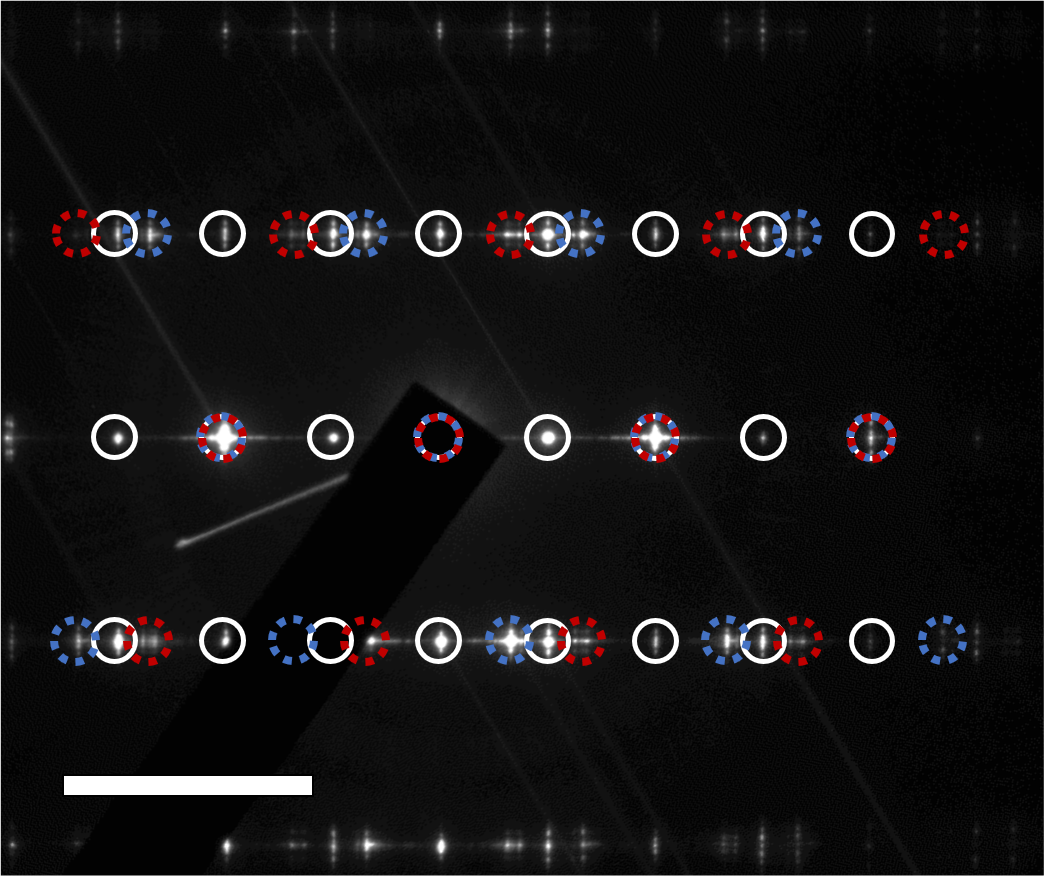
\includegraphics[width=0.24\linewidth]{Image_46_4}}
		\subcaptionbox{\label{fig:Image_46_5}}{%
		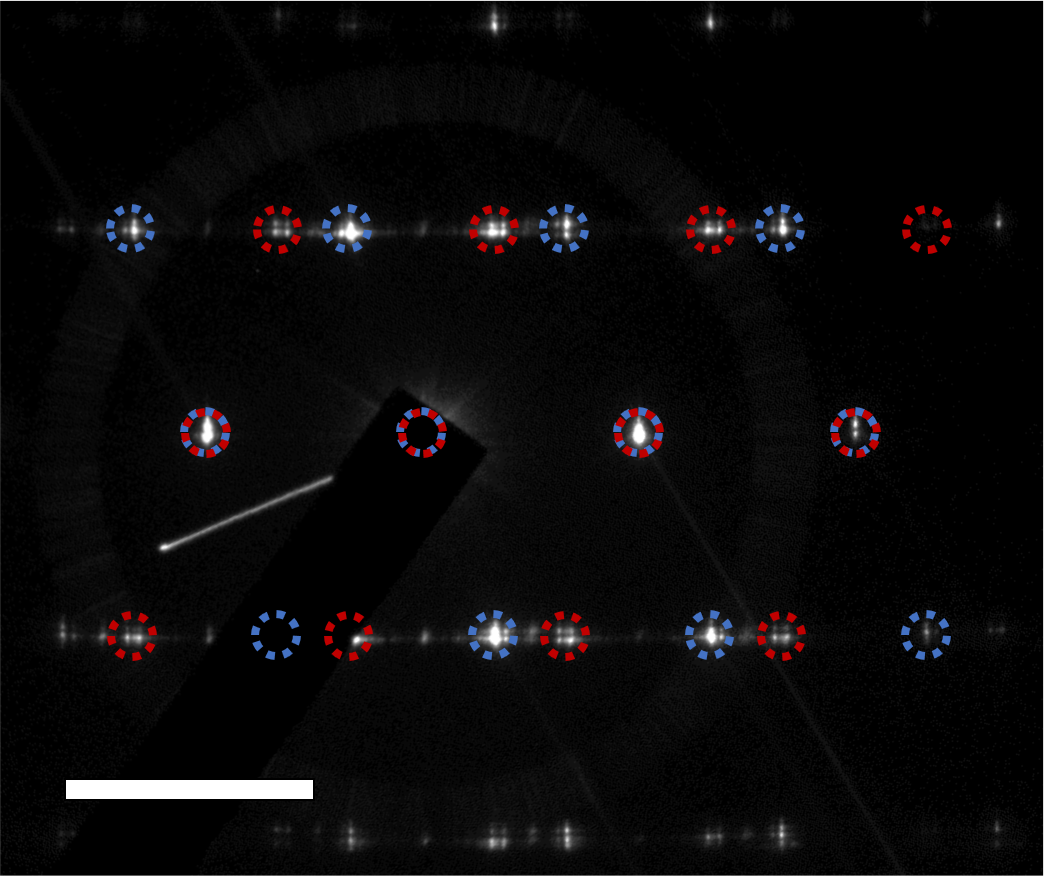
\includegraphics[width=0.24\linewidth]{Image_46_5}}
		\subcaptionbox{\label{fig:Image_46_6}}{%
		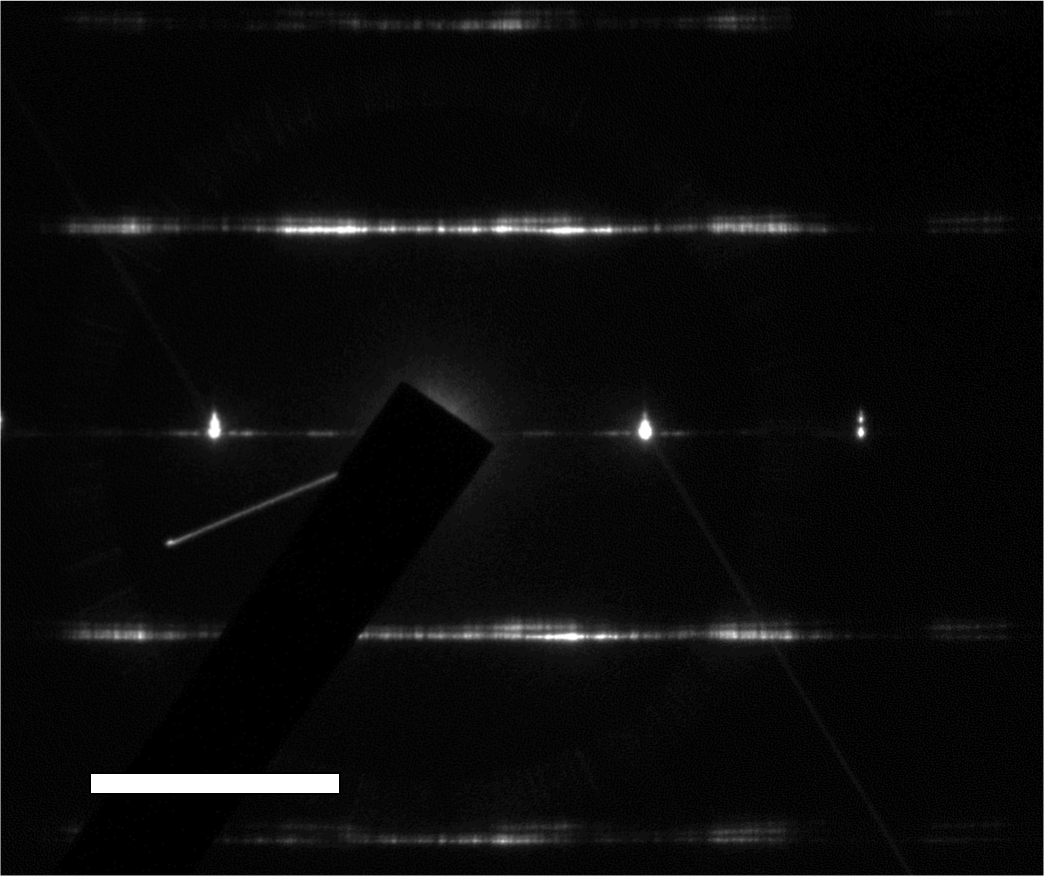
\includegraphics[width=0.24\linewidth]{Image_46_6}}

		температура роста 640\si{\degreeCelsius};

		первая стадия: рост 2000~\si{\second} при ЭДП P/Ga 30;

		вторая стадия: рост 5000~\si{\second} при ЭДП P/Ga 12;

		\subcaptionbox{\label{fig:Image_46_7}}{%
		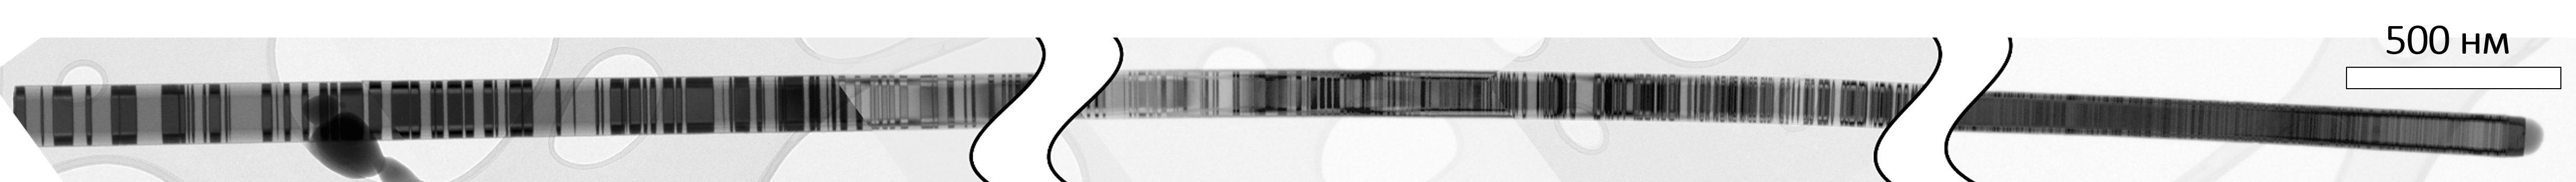
\includegraphics[width=1\linewidth]{Image_46_7}} } \legend{ННК
		ориентированы вершиной направо. Положения рефлексов для фаз ZB и WZ
		отмечены синим (ZB), красным пунктиром (ZB двойникование) и сплошными
		белыми кружками (WZ)} \caption{Темнопольные ПЭМ изображения ННК GaP с WZ
		дифракционным контрастом~(a, б). Картины микродифракции из областей,
		отмеченных пунктиром~(в--е).  Светлопольные ПЭМ изображения ННК GaP образца
VIII~(ж)}\label{fig:Image_46} \end{figure}

На темнопольных изображениях ПЭМ с выбором WZ брэгговских отражений
(см.~рис.~\cref{fig:Image_46_1}, \cref{fig:Image_46_2}) наблюдается высокая
плотность дефектов упаковки и границ двойникования, которые выглядят как тонкие
светлые линии, расположенные поперёк оси ННК. Картины электронной
микродифракции с ориентацией образца вдоль оси зоны [110] указывают на
двойникование вокруг направления роста <111>\textsubscript{GaP}
(см.~рис.~\cref{fig:Image_46}). Удлинение брэгговских пиков по нормали к
направлению плоскости дефектов наблюдается в области ННК c высокой плотностью
планарных дефектов (см.~рис.~\cref{fig:Image_46_6}).

У основания (слева на~рис.~\cref{fig:Image_46}) и вершины ННК (справа
на~рис.~\cref{fig:Image_46}) находятся включения со структурой WZ (светлый
контраст) (см.~рис.~\cref{fig:Image_46_3}). Можно предположить, что
формирование структуры WZ в верхней части ННК вызвано расходом капли
катализатора при охлаждении образца после роста под потоком P и последующим
уменьшением краевого угла смачивания (подробнее
см.~подраздел~\cref{subsec:ch1/sec2/sub5}).  Образование включений со
структурой WZ у оснований ННК может указывать на то, что угол смачивания
каталитической капли близок к 90{\textdegree} на начальной стадии роста.

Толщина бездефектных сегментов исследованных образцов слабо зависит от
отношения потоков P/Ga и температуры роста. Плотность планарных дефектов
увеличивается к вершине ННК. В зависимости от положения, бездефектный сегмент
может иметь толщину от 1--10~\si{\nano\meter} в середине длины ННК до
100--500~\si{\nano\meter} у основания. Несмотря на то, что наблюдаемый эффект
не зависит от отношения потоков P/Ga (см.~рис.~\cref{fig:Image_46_1},
\cref{fig:Image_46_2}), переход в двухстадийном образце к более низким
отношениям потоков P/Ga способствует более частому образованию двойниковых
дефектов (см.~рис.~\cref{fig:Image_46_6}).

\section{Основные результаты главы}\label{sec:ch5/sec8}

Показано, что капли необходимой для зарождения ННК морфологии (размера и
краевого угла смачивания) могут самоорганизованно формироваться при
одновременном открытии шторок источников Ga и P. В случае предварительного
нанесения Ga уменьшается плотность массива вертикальных ННК.

Метод подготовки поверхностного SiO\textsubscript{x} и его отжига влияет на
смачиваемость поверхности, а следовательно, и на плотность зародышей ННК:
оксид, сформированный в кипящем 1:1:3 растворе
H\textsubscript{2}O\textsubscript{2}:NH\textsubscript{4}OH:H\textsubscript{2}O
приводит к образованию массива с плотностью вертикальных ННК в 2,5 раза выше,
меньшей концентрацией наклонных ННК и островков, по сравнению с оксидом,
подготовленным в кипящем азеотропном растворе
HNO\textsubscript{3}:H\textsubscript{2}O. Последующий отжиг подложки в ростовой
камере позволяет частично десорбировать поверхностный оксид, что приводит к
увеличению плотности массива ННК. Отжиг с удалением оксида препятствует
зарождению ННК.

Плотность вертикальных ННК немонотонно зависит от отношения потоков P/Ga:
зависимость прямая в диапазоне низких значений и обратная в диапазоне высоких
значений. Повышение температуры может эффективно подавлять зарождение наклонных
ННК, а снижение потока Ga~--- паразитных островков.

Показана возможность стимуляции роста боковых граней ННК на уже сформированном
массиве изменением параметров роста так, чтобы увеличить размер капли
катализатора. При этом вынужденный радиальный рост однороден по длине ННК.
Данный эффект однородного радиального роста может быть связан со встраиванием
адатомов в край атомной ступени на боковых гранях ННК, который приводит к росту
в режиме течения ступеней от верхней грани к основанию и радиальному росту с
сохранением толщины по длине ННК.

\FloatBarrier
